\documentclass{article}\usepackage[]{graphicx}\usepackage[]{xcolor}
% maxwidth is the original width if it is less than linewidth
% otherwise use linewidth (to make sure the graphics do not exceed the margin)
\makeatletter
\def\maxwidth{ %
  \ifdim\Gin@nat@width>\linewidth
    \linewidth
  \else
    \Gin@nat@width
  \fi
}
\makeatother

\definecolor{fgcolor}{rgb}{0.345, 0.345, 0.345}
\newcommand{\hlnum}[1]{\textcolor[rgb]{0.686,0.059,0.569}{#1}}%
\newcommand{\hlstr}[1]{\textcolor[rgb]{0.192,0.494,0.8}{#1}}%
\newcommand{\hlcom}[1]{\textcolor[rgb]{0.678,0.584,0.686}{\textit{#1}}}%
\newcommand{\hlopt}[1]{\textcolor[rgb]{0,0,0}{#1}}%
\newcommand{\hlstd}[1]{\textcolor[rgb]{0.345,0.345,0.345}{#1}}%
\newcommand{\hlkwa}[1]{\textcolor[rgb]{0.161,0.373,0.58}{\textbf{#1}}}%
\newcommand{\hlkwb}[1]{\textcolor[rgb]{0.69,0.353,0.396}{#1}}%
\newcommand{\hlkwc}[1]{\textcolor[rgb]{0.333,0.667,0.333}{#1}}%
\newcommand{\hlkwd}[1]{\textcolor[rgb]{0.737,0.353,0.396}{\textbf{#1}}}%
\let\hlipl\hlkwb

\usepackage{framed}
\makeatletter
\newenvironment{kframe}{%
 \def\at@end@of@kframe{}%
 \ifinner\ifhmode%
  \def\at@end@of@kframe{\end{minipage}}%
  \begin{minipage}{\columnwidth}%
 \fi\fi%
 \def\FrameCommand##1{\hskip\@totalleftmargin \hskip-\fboxsep
 \colorbox{shadecolor}{##1}\hskip-\fboxsep
     % There is no \\@totalrightmargin, so:
     \hskip-\linewidth \hskip-\@totalleftmargin \hskip\columnwidth}%
 \MakeFramed {\advance\hsize-\width
   \@totalleftmargin\z@ \linewidth\hsize
   \@setminipage}}%
 {\par\unskip\endMakeFramed%
 \at@end@of@kframe}
\makeatother

\definecolor{shadecolor}{rgb}{.97, .97, .97}
\definecolor{messagecolor}{rgb}{0, 0, 0}
\definecolor{warningcolor}{rgb}{1, 0, 1}
\definecolor{errorcolor}{rgb}{1, 0, 0}
\newenvironment{knitrout}{}{} % an empty environment to be redefined in TeX

\usepackage{alltt}
\usepackage{hyperref}
\usepackage{blindtext}
\usepackage{graphicx}
\usepackage{float}
\usepackage[a4paper, total={6in, 8in}]{geometry}

\title{Data Visualisation: Theory and Practice}
\author{Yujie Chu, Pia Fullaondo, Qinqing Li, Jacko Zhou}
\IfFileExists{upquote.sty}{\usepackage{upquote}}{}
\begin{document}



\maketitle 
\tableofcontents
\newpage 

\section{Introduction}

\subsection{Motivation and Background}
Motivations for having Data Visualisations - Case Example 1
\\  
\\Florence Nightingale was not only a social reformer and the founder of modern nursing but also a pioneering statistician. It was her application of data visualisation during the Crimean War that transformed the field of healthcare and pushed for social reform.
\\  
\\During the Crimean War, Nightingale recognised that unsanitary hospital conditions were claiming more lives than the battlefield itself. With the help of William Farr, Nightingale created the coxcomb aimed to illustrate the toll of preventable mortality on soldiers, as shown in Figure \ref{fig:coxcomb}.
\\  
\begin{figure}[H]
    \centering
    \includegraphics[width=0.7\textwidth]{Nightingale-mortality.jpg}
    \caption{``Diagram of the causes of mortality in the army in the East", in 1858 by Florence Nightingale}
    \label{fig:coxcomb}
\end{figure}
\\  
\\The coxcomb, resembling an unconventional pie chart, partitioned mortality by causes. Blue indicates preventable deaths, red indicates deaths by wounds, and black indicates other causes.
The blue areas outweighed the red and black sections combined, highlighting the disproportionate impact of unsanitary hospital conditions on the mortality rate.
\\   
\\Nightingale leveraged the compelling visualisations in her advocacy efforts, presenting them to MPs and government officials who otherwise are unlikely to read or understand statistical reports. Nightingale successfully persuaded Queen Victoria, head of the British Army at the time, to allocate funding for the improvement of better conditions in military hospitals.
\\  
\\Motivations for having Data Visualisations - Case Example 2
\\  
\\Sometimes, one glance is enough to convey the most powerful idea. Edward Hawkins, a British climate scientist and Professor of climate science at the University of Reading, is renowned for his exceptional data visualizations of climate change.
\\ 
\\In 2018, Edward Hawkins was invited to deliver a lecture on climate change in Wales to an audience with diverse backgrounds. It was important to effectively convey the growing urgency surrounding global warming. To achieve this, he created a chart that used just colours, without any words, titles, or legends, as shown in Figure \ref{fig:global}. This seemingly simple yet remarkably powerful chart visually illustrated the Earth's warming trend since 1850.
\begin{figure}[H]
    \centering
    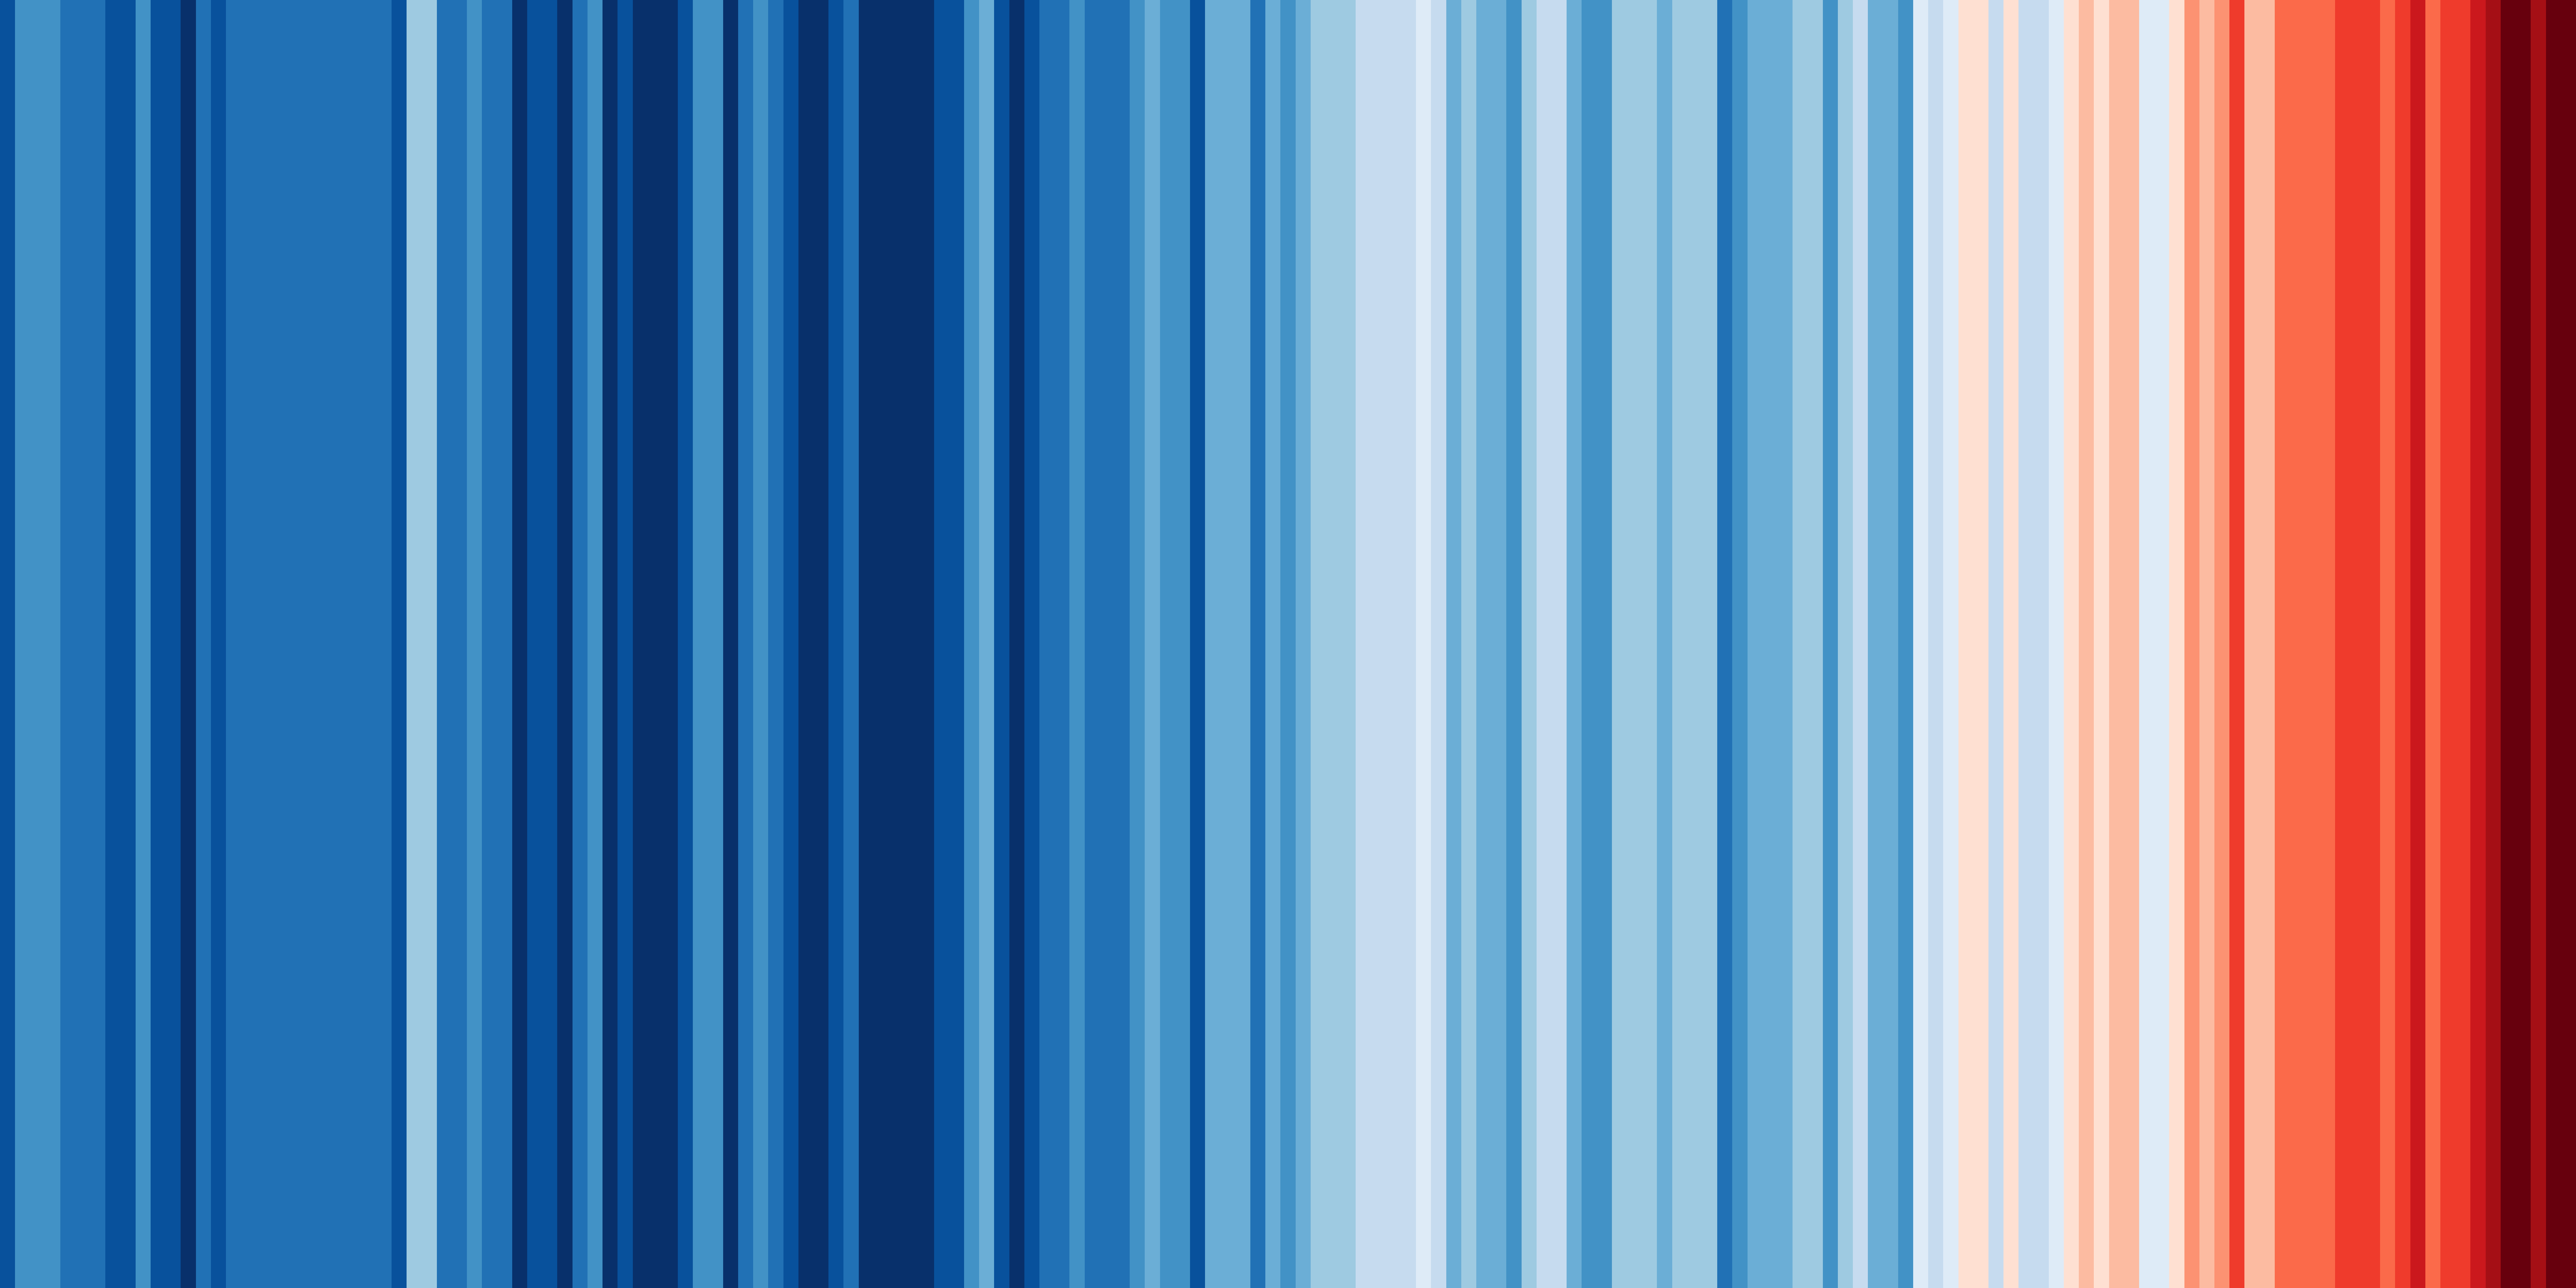
\includegraphics[width=0.7\textwidth]{global.png}
    \caption{``Latest global stripes (1850-2020)", by Edward Hawkins}
    \label{fig:global}
\end{figure}
\\Known as the ``warming stripes," this chart cleverly employs blues to indicate cooler-than-average years and reds to signify hotter-than-average years. Its influence reached far and wide, gracing the front pages of major media outlets and featured in news broadcasts worldwide. It became a symbol in climate change demonstrations. Arguably, it stands as one of the most iconic graphics in modern times.
\\  
\\  
\\Misuses of Data Visualisation - Case Example 1
\\  
\\Inappropriate data visualization conceals trends rather than revealing them. Figure \ref{fig:misuse1} illustrates an instance of this issue. On the left-hand side, an inappropriate scale was used --- the y-scale ranging from 0 to 30 million dollars, obscuring the fluctuations in payroll spending. Conversely, on the right-hand side, observe that there's a significant increase of over 500,000 dollars in just two months. This revelation is substantial; considering inflation, 500,000 dollars in 1937 is worth well over 10 million dollars today.
\begin{figure}[H]
    \centering
    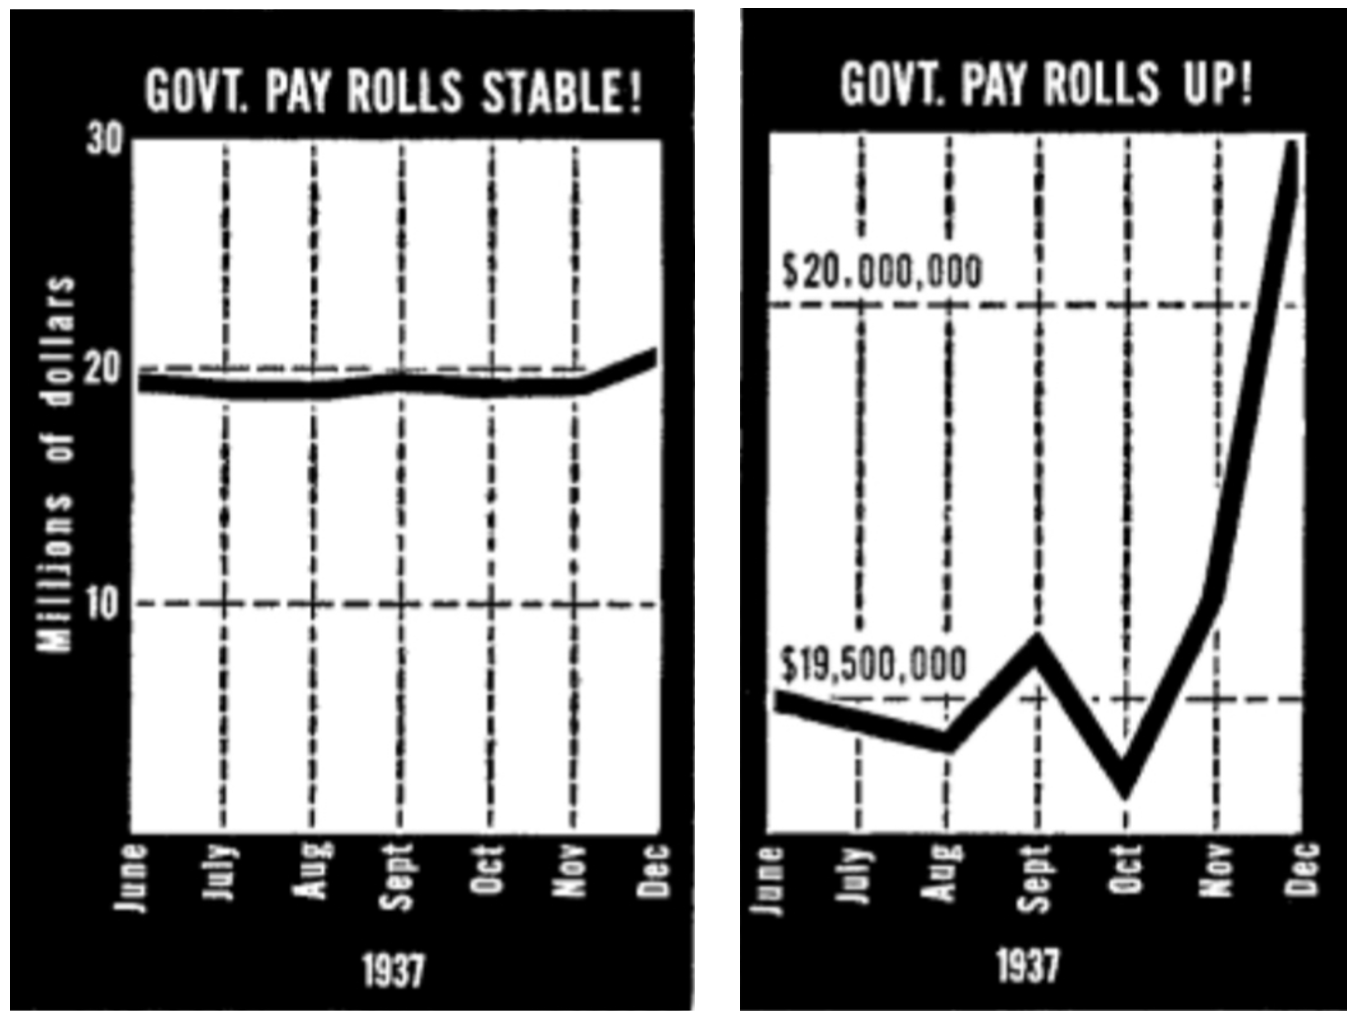
\includegraphics[width=0.7\textwidth]{misuse1.png}
    \caption{Inappropriate use of data visualisation}
    \label{fig:misuse1}
\end{figure}
\\
\\Misuses of Data Visualisation - Case Example 2
\\  
\\Data visualization can be misused, leading to disastrous consequences. One striking example of such misuse is found in the Kallikak Family tree, which was one of the most prominent eugenic narratives of the 20th century.
\\  
\\The visualization (as shown in Figure \ref{fig:familytree}) was created by the psychologist Henry Goddard and presented in his 1912 book, ``The Kallikak Family: A Study in the Heredity of Feeble-Mindedness." Goddard's narrative centered around Martin Kallikak, a soldier who, in addition to his marriage to a respected citizen, had a one-night stand with a ``feeble-minded" maid. Goddard believed that intellectual disabilities were inherited traits. In Goddard's account, the legitimate family was successful, while the children of the ``feeble-minded" maid were labeled as "the lowest types of human beings." However, research has since revealed that the entire story was fictitious, as there was no record of the maid's existence.
\\  
\\Regrettably, the Kallikak family tree became a central element in the eugenics movement for decades afterward. It was featured in the 1935 Nazi propaganda film ``Das Erbe" (The Inheritance), which was used to promote public acceptance of Nazi eugenics laws. This propaganda laid the groundwork for the forced sterilization of approximately 400,000 people under Nazi eugenics policies.

\begin{figure}[H]
    \centering
    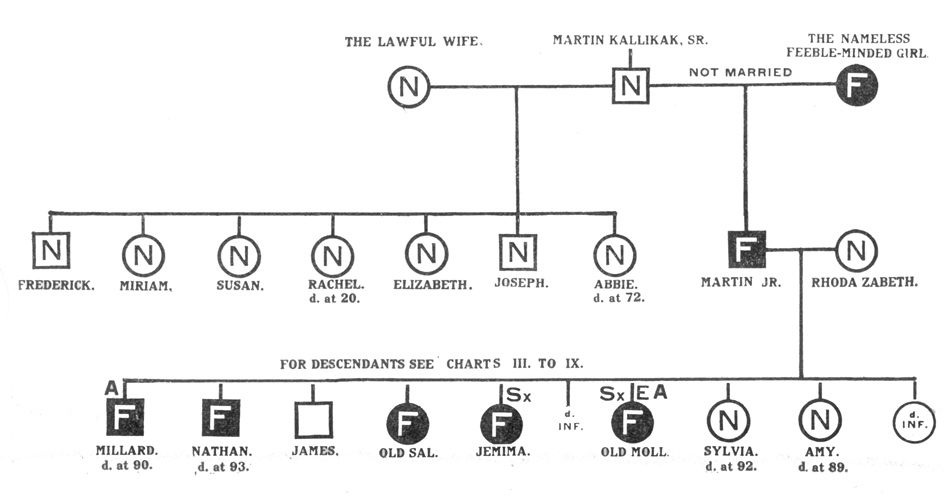
\includegraphics[width=0.7\textwidth]{familytree.jpg}
    \caption{The Kallikak Family tree, in 1912 by Henry Goddard }
    \label{fig:familytree}
\end{figure}

\subsection{Computing and Data Visualisation}
XXX

\subsection{Dataset}
In this section, we unveil the datasets used throughout our study. This section delves into the comprehensive depiction of the diverse datasets employed. Each dataset is meticulously introduced, elucidating its source, structure, and relevance to our investigation.\\

\noindent
\textbf{The Mtcars dataset}: The \textit{Mtcars} dataset, available as a built-in dataset in R, offers a glimpse into the automotive world of the early 1970s. This dataset encompasses 11 attributes for 32 distinct car models. Some of the variables included are: Miles per Gallon (mpg), Number of cylinders (cly), Horsepower (hp), and Weight of the car in tons (wt).\\

\noindent
\textbf{The annual fire in Brazil dataset}: The Fire Information for Resource Management System (FIRMS) provides Near Real-Time (NRT) active fire data from the Moderate Resolution Imaging Spectroradiometer (MODIS), available at NASA. A subset containing historical active fire data of Brazil from 2013 to 2022 contains over 200,000 observations each year was used in this report. This dataset contains 15 variables: latitude: Latitude of active fire data, longitude: Longitude of active fire data, brightness: Brightness of active fire data, scan: Scan resolution, track: Track resolution, acq\_date: Acquisition date, acq\_time: Acquisition time, satellite: Satellite name, instrument: Instrument type, confidence: Confidence level, version: Data version, bright\_t31: Brightness temperature band 31, frp: Fire Radiative Power, daynight: Day or night indicator, type: Fire type.\\

\noindent
\textbf{The Tooth Growth dataset}: \textit{The ToothGrowth dataset}, available as a built-in dataset in R, offers the impact of vitamin C on the tooth growth of Guinea pigs. The dataset consists of 60 observations and 3 variables: len: Length of the Guinea pigs' teeth, supp: Method of vitamin C supplementation, dose: Dose of vitamin C in milligrams per day.\\

\noindent
\textbf{The Edgar Anderson's Iris dataset}: The Anderson's iris data, available as a built-in dataset in R, offers the measurements in centimeters of sepal length and width, petal length and width, along with the species name for 50 flowers from each of three species of iris. The dataset consists of 5 variables: Sepal.Length: Sepal length, Sepal.Width: Sepal width, Petal.Length: Petal length, Petal.Width: Petal width, Species: Species name.\\

\noindent
\textbf{Exchange rate data}: The exchange rate data, available at the Bank of England, provides daily spot exchange rates against GBP over the time period from 2005 to now (without weekends). A subset of daily spot exchange rate of CNY, CAD, EUR, HKD, and USD against GBP from January 2013 to October 2023 was used in this report. The dataset contains 5 variables: Date: Date of spot exchange rate, CNYtoGBP: Spot exchange rate of CNY against GBP, CANtoGBP: Spot exchange rate of CAD against GBP, EURtoGBP: Spot exchange rate of EUR against GBP, HKDtoGBP: Spot exchange rate of HKD against GBP, USDtoGBP: Spot exchange rate of USD against GBP.\\

\noindent
\textbf{Trees dataset}: The trees dataset, available as a built-in dataset in R, offers measurements from 31 felled black cherry trees and provides insights into the relationship between a tree's girth, its height, and the volume of timber it can produce. The dataset contains 3 variables: Girth: The diameter of the tree, Height: The height of the tree, Volume: The volume of timber that the tree can produce.\\

\subsection{Structure and Organisation of the Thesis}
The thesis begins with Chapter 1: "Theoretical Foundations of Data Visualisation", an introductory section that lays the theoretical foundation for the subsequent discussions.\\

The crux of this document, Chapter 2: "Modern Methods of Data Visualisation", conducts a detailed exploration of various modern methods of data visualisation. This chapter offering an in-depth analysis and critical evaluation of their applications, strengths, and limitations.\\

Chapter 3: "Practical Implementation" ventures into the practical application of Python Dash and R Shiny for constructing interactive data visualisation dashboards. Subsequently, Chapter 5: "Case Studies" presents case studies, which serve as practical demonstrations of the efficacy and relevance of the discussed visualisation methods in resolving real-world problems. Finally, Chapter 6 "State-of-the-Art Approaches" critically examines state-of-the-art approaches in data visualisation, highlighting emerging trends, methodologies, and technologies in the field.

\newpage 


\section{Theoretical Foundations of Data Visualisation}
This chapter, "Theoretical Foundations of Data Visualisation," delves into the core principles and concepts that serve as the base of this field. We seek to understand not only the "how" but also the "why" behind the creation of visualisations that captivate and inform.

\subsection{Introduction to Data Visualisation Theory}
Creating effective data visualisations requires a robust theoretical framework underlying every chart, graph, or plot. These theoretical underpinnings not only form the basis of data visualisation but also influence how we represent, perceive, understand, and interpret data.\\ 

\textbf{Guiding Principles for Data Representation}\\
The theoretical framework of data visualisation involves guiding principles dictating visual representation of data. These principles include accuracy, emphasizing faithful reflection of underlying data to reduce distortion or misinterpretation; simplicity, advocating for streamlined visuals to convey information effectively; clarity, ensuring visuals are easily understood without unnecessary complexity; relevance, presenting information pertinent to the message or question addressed; and consistency, maintaining uniform use of visual elements like color coding and labeling throughout a visualisation.\\

\textbf{Theoretical Framework and Visual Perception}\\
Understanding how the human brain processes visual information is a fundamental aspect of data visualisation theory. This knowledge plays a crucial role in designing visualisations that effectively connect with viewers. It encompasses several key considerations: Gestalt Principles, which encompass proximity, similarity, and continuity, affecting how visual elements are grouped and interpreted; Color Theory, involving the strategic use of color contrasts and harmonies to improve clarity and impact; and the management of Cognitive Load, which emphasizes the importance of reducing mental effort needed to process information.\\

\subsection{Visual Perception and Cognition}
Here, we explore human visual perception, along with the application of cognitive psychology principles in data visualisation and highlight the crucial role of pre-attentive attributes in shaping our perception of data.\\ 

\textbf{Human Visual Perception: Decoding Visual Information}\\
Human visual perception, a remarkable cognitive process, profoundly influences our understanding of the surrounding world. When applied to data visualisation, it elucidates how individuals engage with and derive meaning from visual data representations. Significant aspects of human visual perception within data visualisation encompass pattern recognition, adept at identifying trends, outliers, and relationships in data representations. Additionally, perceptual grouping, where visually similar elements are grouped together, influences the interpretation of data clusters and shapes. Moreover, the hierarchy of perception dictates that certain visual attributes are processed more swiftly and effectively than others, such as color being processed faster than text, influencing the viewer's attention hierarchy.\\

By harnessing the principles of human visual perception, applying insights from cognitive psychology, and leveraging pre-attentive attributes, data visualisation designers can create visualisations that are not only aesthetically pleasing but also cognitively efficient.	

\subsubsection{The Gestalt Principles}
This section provides an overview of Gestalt principles in visual perception and design, focusing on their relevance to data visualisation and strategies for creating more effective visualisations. Key Gestalt principles crucial in shaping visual information perception include proximity, which groups related elements, similarity that links similar attributes, continuity aiding trend representation, closure for implying connections, and symmetry for balance and aesthetics in visualisations.\\

\textbf{Application of Gestalt Principles in Designing Visualisations}\\
Leveraging Gestalt principles in data visualisation design enhances intuitive and effective information communication. Designers strategically employ these principles to group related data for clarity, minimize visual clutter, use color or shape to denote meaningful categories, establish smooth visual paths guiding the viewer's gaze, and imply connections or patterns within complex datasets.


\subsection{Data abstraction and Representation}
The transformation of raw data into meaningful representations is a pivotal step in data visualisation. This process, known as data abstraction, involves distilling complex datasets into visual forms that convey insights. In this section, we explore data abstraction, the hierarchies and levels of abstraction in data visualisation, and the critical trade-offs between abstraction and the potential loss of information.

\subsubsection{Data Abstraction: Transforming Raw Data}
Data abstraction involves simplifying and structuring raw data into comprehensible and insightful formats. This process serves as the bridge, transforming numbers, text, and variables into visual elements that convey patterns, trends, and relationships, forming the core of informative data visualisations.

\subsubsection{Hierarchies and Levels of Abstraction}
In data visualisation, abstraction operates on multiple levels of granularity. Hierarchies of abstraction allow us to represent data at varying levels of detail: 
\begin{enumerate}
    \item \textbf{Low-Level Abstraction}: At the lowest level, raw data is preserved in its most detailed form. This might include individual data points, measurements, or unprocessed text.
    \item \textbf{Mid-Level Abstraction}: As we move up the hierarchy, data is grouped or aggregated to provide a broader overview. For example, hourly data points may be aggregated into daily or weekly averages.
    \item \textbf{High-Level Abstraction}: At the highest level, data is represented in a condensed and abstracted form, often as summary statistics or key insights. This level provides a big-picture view.
\end{enumerate}

\textbf{Trade-offs Between Abstraction and Information Loss}\\
While abstraction simplifies complex data, it presents trade-offs. Designers of data visualisation must strike a balance between clarity and detail, generalization and specificity, and context versus precision. Abstraction increases clarity but may sacrifice crucial detailed information necessary for some analytical tasks. It offers a more generalized view accessible to a wider audience but might overlook specific nuances essential for experts. While providing valuable context, high-level abstraction may lack the precision required for precise decision-making.\\ 

In data visualisation, the art of data abstraction lies in finding the right level of detail that effectively conveys the intended message while minimising the risk of information loss. This balancing act is a critical consideration in the design of informative and meaningful data visualisations.


\subsection{Data Types and Visualisation Techniques}
In the world of data visualisation, understanding the nature of your data is key. Data comes in various types, and selecting the appropriate visualisation technique is contingent upon recognising these distinctions. In this section, we categorise data types, and demonstrate how to match each data type with suitable visualisation techniques.

\subsubsection{Categorisation of Data Types}
Data types can be broadly categorised into four main types: 
\begin{itemize}
    \item \textbf{Nominal data}: nominal data represents categories or labels without any inherent order. Examples include colours, gender categories, and city names. 
    \item \textbf{Ordinal data}: ordinal data implies a meaningful order or ranking among categories but lacks equal intervals between them. Examples include survey responses (eg. “very satisfied”, “satisfied”, “neutral”, “dissatisfied”, “very dissatisfied”)
    \item \textbf{Interval data}: interval data possesses ordered categories with equal intervals between them, but it lacks a true zero point. Temperature is measured in Celsius or Fahrenheit as an example. 
    \item \textbf{Ratio data}: ratio data includes ordered categories with equal intervals and a meaningful zero point. Examples are age, income, and weight. 
\end{itemize}

\subsubsection{Matching Data Types with Appropriate Visualisation Techniques}
Selecting appropriate visualisation techniques is essential for effective data communication. Various data types demand specific visualisation methods for optimal representation. For nominal data, bar charts and stacked bar charts are effective in displaying categorical information and relative proportions. Ordinal data benefits from ordered bar charts, dot plots, or stacked bar charts, maintaining the ranking and order of categories. Interval data is best visualised using line charts, histograms, and box plots, showcasing trends and distributions without assuming a true zero point. Ratio data finds effective representation through scatter plots, histograms, and line charts, enabling precise comparisons and measurements due to the presence of a meaningful zero point.


\subsection{Colour Theory in Data Visualisation}
Here, we explore the significance of colour in data visualisation, the principles of colour perception and encoding, and the importance of avoiding misleading visualisations through thoughtful colour choices.\\

\textbf{The Importance of Colour in Conveying Information}\\
Color significantly enhances the impact and comprehension of data visualisations. It serves multiple purposes: distinguishing data points, emphasizing trends, and offering contextual information. It is utilized to encode categorical data, differentiating between various groups with distinct colors, and to represent quantitative data by utilizing color intensity or gradients to portray values or magnitudes. Additionally, color is instrumental in adding context to visualisations through background elements, labels, or annotations, imparting meaning to the data.\\

\textbf{Colour Perception and Colour Encoding in Visualisations}\\
Understanding color perception in data visualisation is crucial. Key principles involve considering color discrimination, ensuring accessibility for individuals with color vision deficiencies. Careful selection of color schemes aligned with the intended message is essential—for instance, using warm colors like red and orange to indicate caution or warmth, and cool colors like blue and green to convey calmness or coldness. Additionally, attention should be paid to how colors interact when combined; certain combinations might create visual vibrations or impact text legibility.\\

\textbf{Avoiding Misleading Visualisations Due to Colour Choices}\\
Misleading visualisations often stem from inappropriate or deceptive use of color, requiring precautions to prevent such occurrences. First, maintaining consistency in color usage throughout the visualisation is essential. Employing a uniform color scheme for similar data categories or elements helps establish coherence and understanding. Furthermore, it's crucial to avoid color choices that could distort or exaggerate the data. Overly intense or contrasting colors might mislead interpretations, emphasizing the necessity for judicious color selection.\\
Additionally, providing a clear and concise legend becomes imperative to explain the meaning of colors, especially when dealing with complex or unfamiliar color schemes. A comprehensive legend helps viewers decipher the represented data accurately. User testing stands as another crucial step in the process. Conducting thorough user testing ensures that the chosen color palette effectively conveys the intended message without confusion or misleading the audience. This step validates the visual interpretation and aids in making necessary adjustments to enhance clarity and accuracy in data representation.\\

\subsection{Theoretical Properties of Visualisations}
Effective data visualisation extends beyond aesthetically pleasing graphics; it involves adhering to crucial theoretical properties that enhance expressiveness, precision, accuracy, and scalability in visual representations. This section examines key properties such as expressiveness, effectiveness, the data-ink ratio, principles of minimal ink, as well as precision, accuracy, and scalability.\\

To begin with, we'll define the key concepts that frame this section:
\begin{itemize}
    \item \textbf{Expressiveness}: Visualisations should be expressive, meaning they should effectively communicate the intended message or insights within the data. Expressive visualisations capture the richness and complexity of the underlying data, revealing patterns, trends, and relationships.
    \item \textbf{Effectiveness}: An effective visualisation is one that successfully conveys information to its audience. It allows viewers to understand the data, draw meaningful conclusions, and make informed decisions based on the presented information.
\end{itemize}

\subsubsection{Data-Ink Ratio and the Principle of Minimal Ink} 
This \textbf{Data-Ink Ratio principle}, introduced by Edward Tufte, emphasises maximising the ink (or pixels in digital formats) used to represent the actual data while minimising non-essential ink. A higher data-ink ratio results in a cleaner, more efficient visualisation that reduces clutter and enhances comprehension.\\
The \textbf{Principle of Minimal Ink} builds on the data-ink ratio. This principle advocates for the removal of any visual elements that do not contribute to the viewer's understanding of the data. Eliminating unnecessary ink (e.g., excessive gridlines or decorations) simplifies the visualisation without sacrificing its effectiveness.\\

\textbf{Precision, Accuracy, and Scalability}\\
The concepts that can be mobilised in order to comply by these principles are precision, accuracy, and scalability. Specifically in the context of data visualisation, precision involves striking a balance between presenting sufficient detail for accurate interpretation while avoiding overwhelming complexity. Accuracy is also vital as its role is ensuring faithful representation of true data values to prevent misleading conclusions. Scalability addresses a visualisation's adaptability to varying data sizes and resolutions, demanding the capability to represent both small and large datasets without compromising clarity or performance.

\subsection{Cognitive Load and Visual Complexity}
In data visualisation, achieving a balance between complexity and cognitive load is crucial. This section explores the concept of cognitive load in visualisations, strategies to reduce cognitive load while maintaining complexity, and techniques to combat information overload through simplification.\\

\textbf{Exploring the Concept of Cognitive Load in Visualisations}\\
In data visualisations, cognitive load significantly influences how viewers engage with and comprehend presented data. Striking a balance is crucial to effectively convey information without overwhelming the viewer's cognitive capacity.

\subsubsection{Strategies to Reduce Cognitive Load While Maintaining Complexity}
To reduce cognitive load while maintaining complexity in data visualisation, several strategies can be employed. Firstly, establishing a clear visual hierarchy using size, color, and contrast helps direct attention to crucial elements. Additionally, simplifying labels and text by avoiding unnecessary complexity and jargon ensures information is clear and easily digestible. Employing interactive features like tooltips and drill-down functionality assists in providing additional information when required, reducing the density of static visualisations. Another approach involves the use of progressive disclosure, presenting complex information gradually, beginning with an overview and allowing users to explore details as needed. Lastly, considering data aggregation where appropriate can help summarize information and alleviate the cognitive load associated with interpreting intricate details.\\

These strategies aim to maintain complexity while lessening the cognitive burden on viewers by directing attention effectively, simplifying content, offering interactive elements, gradually revealing information, and summarizing data where feasible.

\subsubsection{Information Overload and Simplification Techniques}
Addressing information overload in visualisations necessitates the strategic application of simplification techniques. Filtering enables focused data selection, while data reduction aggregates information to highlight overarching trends. Storyboarding structures data presentation, aiding in contextual comprehension, and prioritization ensures critical information is prominently displayed, elevating the visualisation's clarity and impact. These strategies collectively combat overwhelming data or excessive visual elements, enhancing comprehension and the effective communication of insights to viewers.


\newpage

\section{Modern Methods of Data Visualisation}
In this chapter, we explore a variety of powerful visualisation methods, from classic scatter plots and bar charts to advanced techniques like heatmaps and network graphs. Through vivid examples, we'll show when and why each method is used, and delve into the theoretical and mathematical foundations that empower these visualisations to unveil insights hidden within the data.

\subsection{Scatter Plots and Bubble Charts}
Scatter plots and bubble charts are fundamental data visualisation techniques that provide valuable insights into the relationships and patterns within datasets. These visualisations are particularly effective for representing discrete data through data points, since this bring out easily identifiable comparisons, and reveals trends.

\subsubsection{Scatter Plots}
Scatter plots, also known as dot charts or dot density plots, offer a straightforward yet mathematically intriguing method for visualizing data. At their core, they display individual data points as dots along a single axis, where each dot representing a single observation.\\ 
\\The mathematical interest of dot plots lies in their ability to provide a simple visual representation of data distribution, center, and spread. While they don't rely on complex equations or statistical principles, dot plots make it easy to observe important characteristics of data, such as the mode (the most frequent value), skewness (asymmetry), and potential outliers. \\ 
\\They're particularly useful for comparing multiple data sets, identifying patterns, and detecting data irregularities. Their simplicity is what makes dot plots a valuable tool for both introductory statistics education and exploratory data analysis.

\subsubsection{Regression and the Regression Line}
\textbf{Linear regression} is a fundamental statistical method used to model the relationship between a dependent variable (often denoted as \(Y\)) and one or more independent variables (commonly denoted as \(X\)). The objective of linear regression is to find a linear equation that best represents this relationship. In simple linear regression, with one independent variable, the linear regression line is expressed as:

\[
Y = \beta_0 + \beta_1X + \epsilon
\]

Here, \(\beta_0\) is the intercept, \(\beta_1\) is the slope, \(X\) is the independent variable, and \(\epsilon\) represents the error term. The objective of the linear regression line is to minimise the sum of squared differences between the observed and predicted values of \(Y\), which helps us understand how changes in \(X\) affect \(Y\).\\
Linear regression lines are often featured in scatter plots to give readers more insight into the dataset being plotted, by representing the overall relationship between variables and, by allowing them to make quick comparisons between individual observations and the regression line.\\


\textbf{Scatter Plots in Practice}\\
In this example, we'll create a scatter plot that visualises the relationship between two variables - the weight of cars and the amount of miles traveled per gallon of petrol. We'll use the "mtcars" R dataset.

\begin{knitrout}
\definecolor{shadecolor}{rgb}{0.969, 0.969, 0.969}\color{fgcolor}\begin{kframe}
\begin{alltt}
\hlcom{# Create a scatter plot of car weight vs MPG from mtcars dataset}
\hlkwd{library}\hlstd{(ggplot2)}
\hlkwd{ggplot}\hlstd{(}\hlkwc{data} \hlstd{= mtcars,} \hlkwd{aes}\hlstd{(}\hlkwc{x} \hlstd{= wt,} \hlkwc{y} \hlstd{= mpg,} \hlkwc{color} \hlstd{=} \hlkwd{factor}\hlstd{(cyl)))} \hlopt{+}
  \hlkwd{geom_point}\hlstd{(}\hlkwc{size} \hlstd{=} \hlnum{3}\hlstd{,} \hlkwc{alpha} \hlstd{=} \hlnum{0.7}\hlstd{)} \hlopt{+}  \hlcom{# Larger points with transparency}
  \hlkwd{geom_smooth}\hlstd{(}\hlkwc{method} \hlstd{=} \hlstr{"lm"}\hlstd{,} \hlkwc{se} \hlstd{=} \hlnum{FALSE}\hlstd{,} \hlkwc{color} \hlstd{=} \hlstr{"red"}\hlstd{,} \hlkwc{linewidth} \hlstd{=} \hlnum{1}\hlstd{)} \hlopt{+}  \hlcom{# Linear regression trend line}
  \hlkwd{labs}\hlstd{(}
    \hlkwc{x} \hlstd{=} \hlstr{"Weight (1000 lbs)"}\hlstd{,}
    \hlkwc{y} \hlstd{=} \hlstr{"Miles per Gallon"}\hlstd{,}
    \hlkwc{color} \hlstd{=} \hlstr{"Cylinders"}
  \hlstd{)} \hlopt{+}
  \hlkwd{scale_color_manual}\hlstd{(}\hlkwc{values} \hlstd{=} \hlkwd{c}\hlstd{(}\hlstr{"4"} \hlstd{=} \hlstr{"grey"}\hlstd{,} \hlstr{"6"} \hlstd{=} \hlstr{"purple"}\hlstd{,} \hlstr{"8"} \hlstd{=} \hlstr{"blue"}\hlstd{))} \hlopt{+}  \hlcom{# Custom color palette}
  \hlkwd{theme_minimal}\hlstd{()}  \hlcom{# Minimalistic theme}
\end{alltt}


{\ttfamily\noindent\itshape\color{messagecolor}{\#\# `geom\_smooth()` using formula = 'y \textasciitilde{} x'}}\end{kframe}\begin{figure}
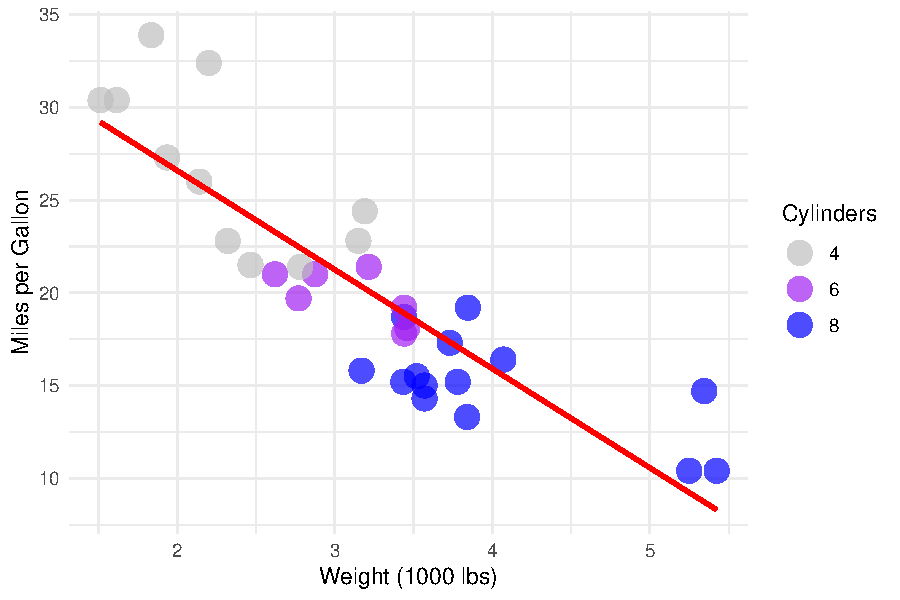
\includegraphics[width=\maxwidth]{figure/scatter-plot-1} \caption[Scatter plot of car weights vs MPG]{Scatter plot of car weights vs MPG}\label{fig:scatter-plot}
\end{figure}

\end{knitrout}

\textbf{Analysis of the scatter plot}\\
Figure~\ref{fig:scatter-plot}, provides insights into the relationship between cars' weight and their MPG, with the added dimension of color-coded cylinders.Particularly it visually highlights and make accessible to the viewer features of the data set, that would otherwise go unnoticed. These are some of the following elements: 
\begin{itemize}
    \item \textbf{Clustering}: The scatter plot reveals distinct clustering of data points, highlighting specific patterns within the dataset. Cars with four cylinders (color "grey") are predominantly clustered in the lower weight and higher MPG region, representing smaller and more fuel-efficient vehicles. In contrast, cars with eight cylinders (color "blue") tend to be clustered in the higher weight and lower MPG area, indicating larger and less fuel-efficient cars. The identification of this clustering aids in visualising how the number of cylinders influences the trade-off between weight and fuel efficiency.\\
    \item \textbf{Linear Regression Line}: The regression line provides a visual representation of the overall relationship between car weight and fuel efficiency.If the line has a positive slope, it indicates that as car weight increases, MPG decreases. Conversely, a negative slope suggests that heavier cars tend to have higher MPG. The steepness of the line represents the strength of this relationship. In this case, the reed regression line indicates a negative correlation—cars tend to have lower fuel efficiency as their weight increases.
\end{itemize}

\subsubsection{Bubble Charts}
Bubble charts are a captivating data visualisation tool that extends beyond the typical two-dimensional scatter plot by introducing an extra dimension. They represent data points as bubbles or circles on a two-dimensional plane, where the size of each bubble encodes a third variable. This technique enhances data visualisation by facilitating the exploration of multivariate data and uncovering patterns that may be hidden in traditional scatter plots.\\

\textbf{Bubble Chart's Utility in Visualising Data}\\
Bubble charts excel in scenarios where three key variables need to be conveyed simultaneously. The x-axis and y-axis represent two variables, as in a standard scatter plot, while the size of the bubble encodes a third variable, often a quantitative one. This allows for the visualisation of relationships between three variables in a single, intuitive graphic.\\
For instance, in economics, bubble charts can illustrate economic indicators, with the x-axis showing time, the y-axis displaying GDP growth, and the bubble size representing a related factor like population or inflation. \\

\textbf{Mathematical Intricacies}\\
The mathematical intricacies of constructing bubble charts involve scaling the data values to determine the size of each bubble accurately. The size of the bubble is typically proportional to the square root of the variable it represents. The choice of scaling method depends on the data distribution and the message the chart aims to convey.

The formula for calculating the bubble size (\(S\)) often involves applying a linear or nonlinear scaling function:

\[
S = k \cdot \sqrt{V}
\]

Where:
\begin{itemize}
\item \(S\) is the size of the bubble,
\item \(V\) is the value of the variable being represented, and
\item \(k\) is a scaling factor to control the bubble size.
\end{itemize}

Selecting an appropriate scaling factor (\(k\)) is critical for maintaining the proportionality between the bubble size and the variable being represented.\\

\textbf{Bubble Charts in Practice}
 This bubble plot visualises data from the same dataset as above. The purpose of this plot is to depict the relationship between car models and their fuel efficiency (mpg) while using the size of the bubbles to represent the car's horsepower (hp) and color-coding the bubbles based on the number of cylinders (cyl).

\begin{knitrout}
\definecolor{shadecolor}{rgb}{0.969, 0.969, 0.969}\color{fgcolor}\begin{kframe}
\begin{alltt}
\hlcom{#Create bubble plot }
\hlkwd{ggplot}\hlstd{(mtcars,} \hlkwd{aes}\hlstd{(}\hlkwc{x} \hlstd{=} \hlkwd{rownames}\hlstd{(mtcars),} \hlkwc{y} \hlstd{= mpg,} \hlkwc{size} \hlstd{= hp,} \hlkwc{color} \hlstd{= cyl))} \hlopt{+}
  \hlkwd{geom_point}\hlstd{()} \hlopt{+}
  \hlkwd{labs}\hlstd{(}
    \hlkwc{x} \hlstd{=} \hlstr{"Car Models"}\hlstd{,}
    \hlkwc{y} \hlstd{=} \hlstr{"Miles per Gallon"}\hlstd{,}
    \hlkwc{size} \hlstd{=} \hlstr{"Horsepower (hp)"}\hlstd{,}
    \hlkwc{color} \hlstd{=} \hlstr{"Cylinders (cyl)"}
  \hlstd{)} \hlopt{+}
  \hlkwd{scale_size_continuous}\hlstd{(}\hlkwc{range} \hlstd{=} \hlkwd{c}\hlstd{(}\hlnum{3}\hlstd{,} \hlnum{10}\hlstd{))} \hlopt{+}
  \hlkwd{scale_color_gradient}\hlstd{(}\hlkwc{low} \hlstd{=} \hlstr{"lightblue"}\hlstd{,} \hlkwc{high} \hlstd{=} \hlstr{"darkblue"}\hlstd{)} \hlopt{+}
  \hlkwd{theme_minimal}\hlstd{()} \hlopt{+}
  \hlkwd{theme}\hlstd{(}\hlkwc{axis.text.x} \hlstd{=} \hlkwd{element_text}\hlstd{(}\hlkwc{angle} \hlstd{=} \hlnum{90}\hlstd{,} \hlkwc{hjust} \hlstd{=}\hlnum{1}\hlstd{))}
\end{alltt}
\end{kframe}
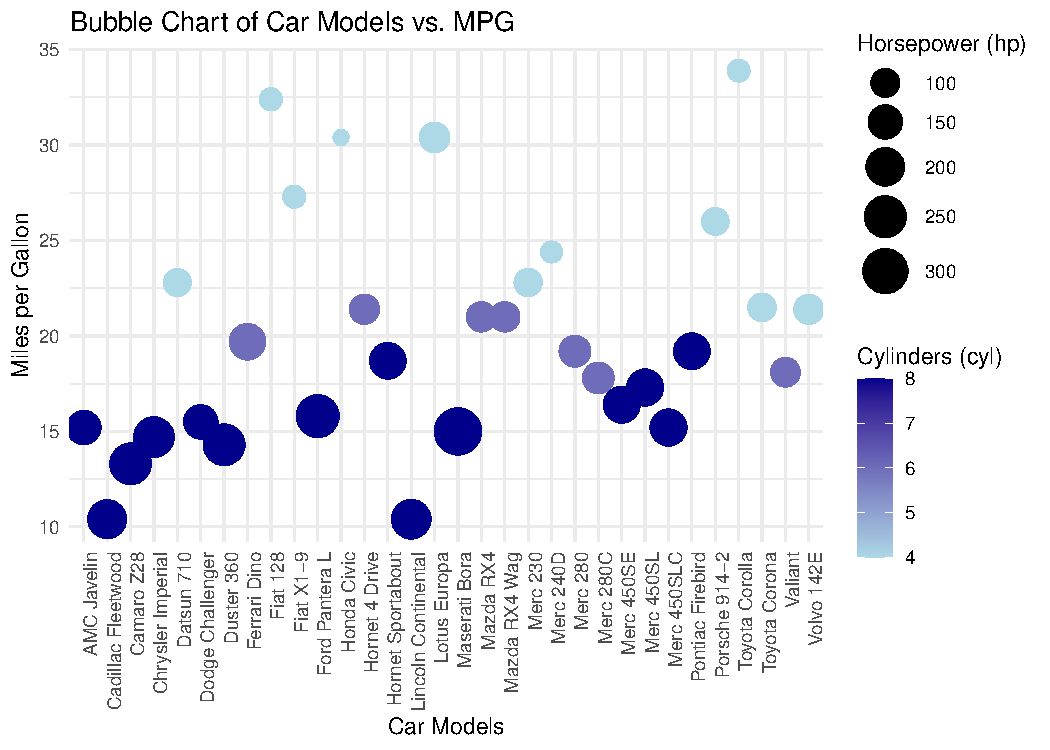
\includegraphics[width=\maxwidth]{figure/buble-plot-chunk-1} 
\end{knitrout}

\textbf{Analysis of the bubble chart}\\
The plot's title, axis labels, and legends provide context and clarity to the visualisation, making it accessible and informative. Additionally, the choice of a gradient color scale for the number of cylinders enhances the visual appeal and aids in interpreting the data.This bubble plot allows for quick comparisons between multiple characteristics of different car models.The resulting bubble plot effectively conveys several key insights:
\begin{enumerate}
\item \textbf{Car Model vs. MPG}: The x-axis displays the car models, offering a clear representation of each vehicle in the dataset. The bubble plot is particularly useful for displaying nominal data, such as car model names, as it allows easy identification and comparison.
\item \textbf{Miles per Gallon (MPG)}: The y-axis measures miles per gallon, representing the fuel efficiency of each car model. Higher bubbles indicate better fuel efficiency. This variable, which is continuous, is positioned vertically to demonstrate how each car model's fuel efficiency relates to others.
\item \textbf{Horsepower (HP)}: The size of each bubble represents the car's horsepower (hp). Larger bubbles correspond to higher horsepower, providing an additional dimension to the data. The size encoding helps identify more powerful cars.
\item \textbf{Cylinders (Cyl)}: The color of each bubble is determined by the number of cylinders (cyl) in the car's engine. The color scheme adds a categorical aspect to the visualisation, making it easy to differentiate between cars with different cylinder counts.
\end{enumerate}


\subsection{Bar Charts and Histograms}
\subsubsection{Bar Charts}
A bar chart is a very important method to present data. It organizes information into vertical bars.  Bar charts have lots of advantages in data visualisation. It can present data categories in a frequency distribution. A bar chart is best for comparing classified data. Especially when the values are close, because the human perception of height is better than other visual elements (such as area, angle, etc.), the use of a bar chart is more appropriate. These bars usually have different lengths, and every length is proportional to the size of the information they present.\\
R uses the function $barplot()$ to create bar charts. R can draw both vertical and Horizontal bars in the bar chart. In the bar chart, each of the bars can be given different colors.\\
R is a programming language for data analysis and statistical computing, and its advent has made data visualisation more straightforward and accessible. Among the various tools available in R, ggplot2 stands out as one of the most renowned and powerful tools for creating data visualisations. It offers a wealth of data visualisation capabilities and is celebrated for its versatility and aesthetic appeal. In this chapter, we will focus on how to use ggplot2 to create bar charts for data visualisation.\\

\subsubsection{Different Types of Bar Charts}
Here is an overview of the different types of bar charts. \\
\paragraph{Vertical Bar Chart}
This is the most common bar chart. We use different vertical columns to display and compare the values of different categories in the same dimension, where the X-axis represents the contrasting categories and the Y-axis represents the frequency or count of their categories.\\
\paragraph{Horizontal Bar Chart}
This is very similar to a vertical bar chart but rotated 90 degrees. Categories are shown on the y-axis and frequency or count are shown on the x-axis. Horizontal bar charts are especially useful when category names are long or when there are numerous categories.
\paragraph{Multi-set Bar Chart}
Also known as a grouped bar chart or clustered bar chart. A multi-set bar chart is used to represent and compare different sub-groups within individual categories. This type of chart is useful when you want to show and compare multiple sets of data side-by-side.
Multi-set Bar charts can be horizontal or vertical like the other normal bar charts, and the length of each bar represents the frequency or count of their categories.
\paragraph{Stacked bar chart}
Similar to bar charts, stacked bar charts are often used to compare different classes of values and, within each class of values, are divided into sub-classes, which are often referred to by different colors. Each segment's size is proportional to the frequency or count that it represents from the sub-category. The entire bar's length represents the cumulative total of all the sub-categories.
However, it is very easy to get confused when there are too many categories.

\textbf{Advantages of Bar Charts:}
\begin{enumerate}
\item \textbf{Clarity and Simplicity}: Bar charts are structurally simple, making them easy to read and understand, allowing audiences to quickly grasp key information.
    \item \textbf{Effective Comparison}: They provide a visual representation that makes comparing the size or value of different categories straightforward, especially when comparing a limited number of categorical data.
    \item \textbf{High Flexibility}: They can be used to represent any type of data, be it continuous or discrete.
    \item \textbf{Multilevel Representation}: Stacked or grouped bar charts can be used to represent multiple data series.
\end{enumerate}

\textbf{Disadvantages of Bar Charts:}
\begin{enumerate}
    \item \textbf{Limited Data Representation}: They might not be suitable for representing large datasets as things can get cluttered.
    \item \textbf{Potential Misinterpretation}: Without a zero baseline, bar charts can be misleading as they might exaggerate differences.
    \item \textbf{Overcomplexity with Many Categories}: If there are too many bars, it can be challenging to discern information effectively.
    \item \textbf{Requires Categorical Data}: Bar charts are not ideal for representing trends over continuous data, where line graphs might be more appropriate.
\end{enumerate}
\subsubsection{ToothGrowth Dataset}


This bar chart below illustrates the tooth growth in relation to varying doses of a vitamin. The key observations are:

\begin{enumerate}
    \item \textbf{X-axis Description:} The X-axis represents different dosages of the vitamin (mg/day). There are three distinct dosage levels.
    
    \item \textbf{Y-axis Description:} The Y-axis signifies the length of tooth growth (len). This represents the average tooth growth at the given vitamin dosage.
    \item \textbf{Data Observation:} From the heights of the bars, it is evident that as the vitamin dosage increases, the tooth growth also appears to increase. This might suggest that higher doses of the vitamin may promote tooth growth.
\end{enumerate}
\begin{figure}[htbp]
  \centering
  \begin{minipage}[b]{0.45\linewidth}
\begin{knitrout}
\definecolor{shadecolor}{rgb}{0.969, 0.969, 0.969}\color{fgcolor}
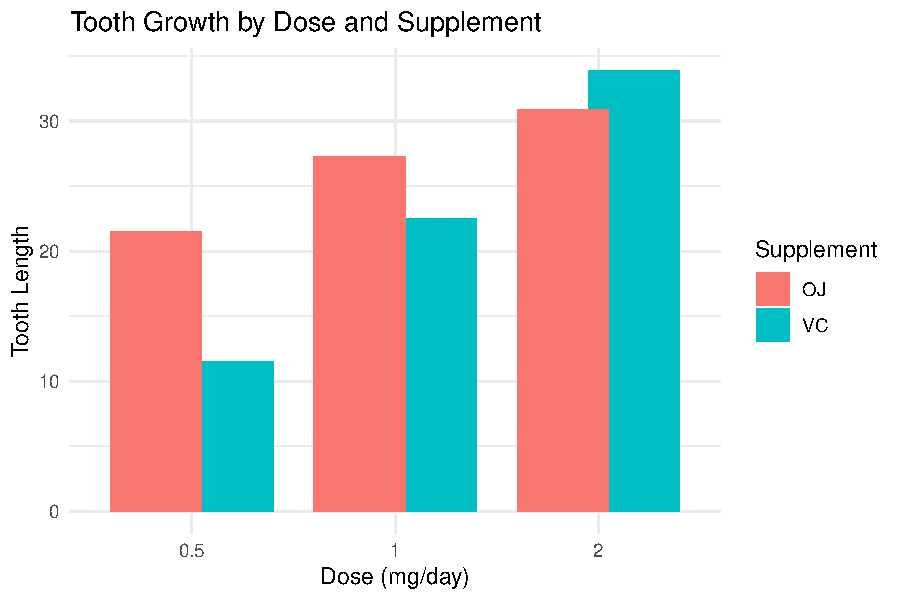
\includegraphics[width=\linewidth]{figure/barchart2-1} 
\end{knitrout}
    \caption{Tooth Growth by Dose and Supplement (grouping bar chart)}
    \label{fig:barchart2}
  \end{minipage}
  \hfill
  \begin{minipage}[b]{0.45\linewidth}
\begin{knitrout}
\definecolor{shadecolor}{rgb}{0.969, 0.969, 0.969}\color{fgcolor}
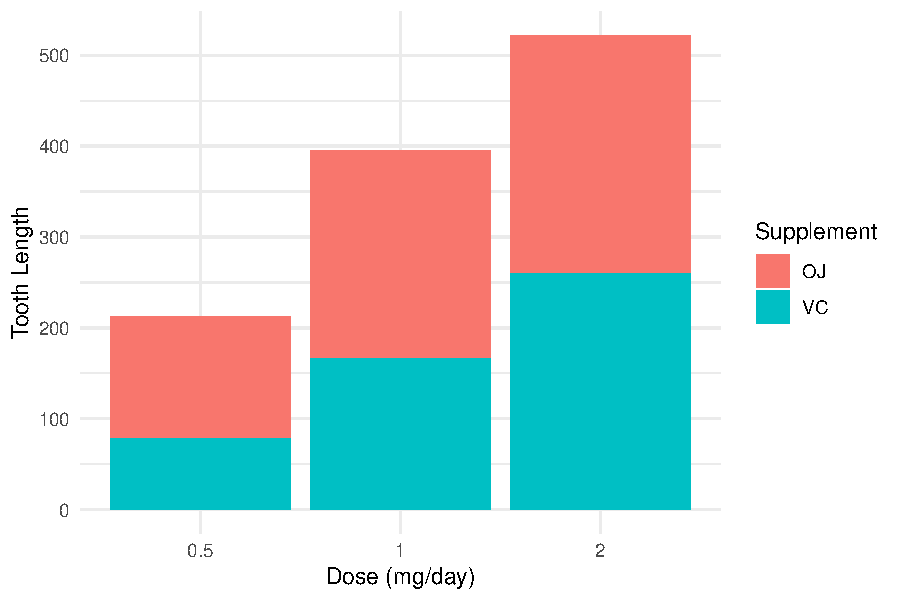
\includegraphics[width=\linewidth]{figure/barchart3-1} 
\end{knitrout}
    \caption{Tooth Growth by Dose and Supplement (stacked bar chart)}
    \label{fig:barchart3}
  \end{minipage}
\end{figure}
The displayed bar chart~\ref{fig:barchart2} provides insights into tooth growth influenced by varying doses of a vitamin, further categorized by the type of supplement (`supp`). The key insights from this chart are:

\begin{enumerate}
    \item \textbf{X-axis Description:} The X-axis demarcates different vitamin dosages, categorized into three distinct levels: 0.5, 1, and 2 mg/day.
    
    \item \textbf{Y-axis Description:} The Y-axis quantifies tooth growth length, representing the combined average growth for both supplements at the respective vitamin dosages.
    \item \textbf{Data Observation:} The total height of each bar signifies the combined tooth growth for both supplements at the given dosage. From the stacked sections, it's evident that the impact on tooth growth varies based on the supplement type. A detailed inspection might elucidate the relative effectiveness of the supplements at each dosage level.
\end{enumerate}
The structure of the second figure~\ref{fig:barchart2} is quite similar to that of the first one, with the main difference lying in the method of data representation. Forming a bar chart, it facilitates the understanding of the combined effects of the two supplements at each dosage level. However, compared to the grouped bar chart, it becomes more challenging to differentiate the individual contributions of each supplement.

In the next part of our section, we will look at another plot which called Histogram.
\subsubsection{Histograms}
Histograms, although visually similar to bar charts, convey different meanings. A histogram involves concepts of statistics. It requires data to be categorized into groups and then counts the data points within each of those groups. On a Cartesian coordinate system, the x-axis shows the endpoints of each group, and the y-axis represents frequency. The height of each rectangle indicates the corresponding frequency, making it a frequency distribution histogram. In order to determine the quantity of each group in the histogram, a multiplication of the frequency by the group interval is necessary. Since every histogram has a fixed group interval, if we use the y-axis to directly show quantity and each rectangle's height indicates the number of data points, we can both retain the distribution and simultaneously see the number in each group at a glance. All examples in this text use the non-standard histogram depiction with the y-axis denoting quantity.

\textbf{Uses of Histograms:}
Histograms demonstrates the distribution of frequency or quantity across groups.\\
Facilitates the visualisation of differences in frequency or quantity among groups.\\
The R language uses the $hist()$ function to create histograms. This function takes vectors as input and uses a few more parameters to plot the histogram.\\
Now, we want to creat a better graph with ggplot2 thanks to the $geom_histogram()$ function and iris dataset.\\
The iris dataset is a classic dataset in the field of statistics. It was introduced by the British biologist Ronald A. Fisher in 1936 as an example of discriminant analysis. The dataset consists of 150 samples from three species of iris flowers: setosa, versicolor, and virginica. For each sample, four features were measured: the lengths and the widths of the sepals and petals, all in centimeters. The dataset is often used for classification tasks to differentiate between the three species based on the given measurements. It has become a standard test case for many classification algorithms and is widely recognized in the data science community.\\
\begin{knitrout}
\definecolor{shadecolor}{rgb}{0.969, 0.969, 0.969}\color{fgcolor}\begin{kframe}
\begin{alltt}
\hlcom{#Create a histogram using ggplot2 for Sepal Length in the Iris dataset}
\hlstd{bar_diagram} \hlkwb{<-} \hlkwd{ggplot}\hlstd{(iris,} \hlkwd{aes}\hlstd{(}\hlkwc{x} \hlstd{= Sepal.Length))} \hlopt{+}
  \hlkwd{geom_histogram}\hlstd{(}
    \hlkwc{binwidth} \hlstd{=} \hlnum{0.2}\hlstd{,}  \hlcom{# Adjust the box width to 0.2 for smaller data sets}
    \hlkwc{fill} \hlstd{=} \hlstr{"grey"}\hlstd{,}
    \hlkwc{color} \hlstd{=} \hlstr{"black"}
  \hlstd{)} \hlopt{+}
  \hlkwd{labs}\hlstd{(}
    \hlkwc{x} \hlstd{=} \hlstr{"Sepal Length/cm"}\hlstd{,}
    \hlkwc{y} \hlstd{=} \hlstr{"Frequency"}
  \hlstd{)} \hlopt{+}
  \hlkwd{theme_minimal}\hlstd{()}
\hlkwd{print}\hlstd{(bar_diagram)}
\end{alltt}
\end{kframe}\begin{figure}
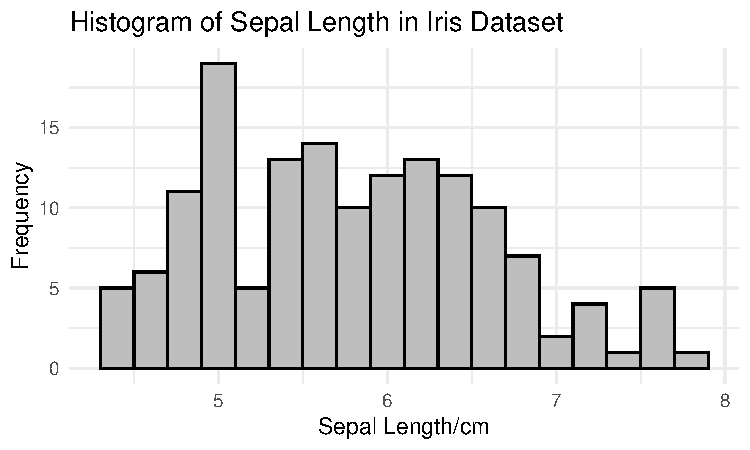
\includegraphics[width=\maxwidth]{figure/hist3-1} \caption[Histogram of Sepal Length in Iris Dataset]{Histogram of Sepal Length in Iris Dataset}\label{fig:hist3}
\end{figure}

\end{knitrout}
\subsubsection{Kernel Density Estimation}
In statistics, Kernel Density Estimation (KDE) is used to infer the distribution of a population based on a limited sample. Thus, the result of the kernel density estimation is an estimate of the sample's probability density function. Based on this estimated probability density function, we can ascertain certain characteristics of the data distribution, such as the regions where data is concentrated.
Here is the expression of KDE euation:
$$\hat{f}(x) = \frac{1}{nh} \sum_{i=1}^{n} K\left(\frac{x - x_i}{h}\right)$$\\
The kernel function \( K(u) \) is a normalized non-negative function that satisfies:
\[ \int K(u) \, du = 1 \]
\begin{knitrout}
\definecolor{shadecolor}{rgb}{0.969, 0.969, 0.969}\color{fgcolor}\begin{kframe}
\begin{alltt}
\hlcom{# Create a Kernel Density Estimate plot using ggplot2 for Sepal Length in the Iris dataset}
\hlstd{kde_diagram} \hlkwb{<-} \hlkwd{ggplot}\hlstd{(iris,} \hlkwd{aes}\hlstd{(}\hlkwc{x} \hlstd{= Sepal.Length))} \hlopt{+}
  \hlkwd{geom_density}\hlstd{(}
    \hlkwc{fill} \hlstd{=} \hlstr{"grey"}\hlstd{,}
    \hlkwc{alpha} \hlstd{=} \hlnum{0.5}\hlstd{,}  \hlcom{# Adjust the transparency for better visualisation}
    \hlkwc{adjust} \hlstd{=} \hlnum{1}  \hlcom{# This parameter can be used to control the smoothness}
  \hlstd{)} \hlopt{+}
  \hlkwd{labs}\hlstd{(}
    \hlkwc{x} \hlstd{=} \hlstr{"Sepal Length/cm"}\hlstd{,}
    \hlkwc{y} \hlstd{=} \hlstr{"Density"}
  \hlstd{)} \hlopt{+}
  \hlkwd{theme_minimal}\hlstd{()}
\hlkwd{print}\hlstd{(kde_diagram)}
\end{alltt}
\end{kframe}\begin{figure}
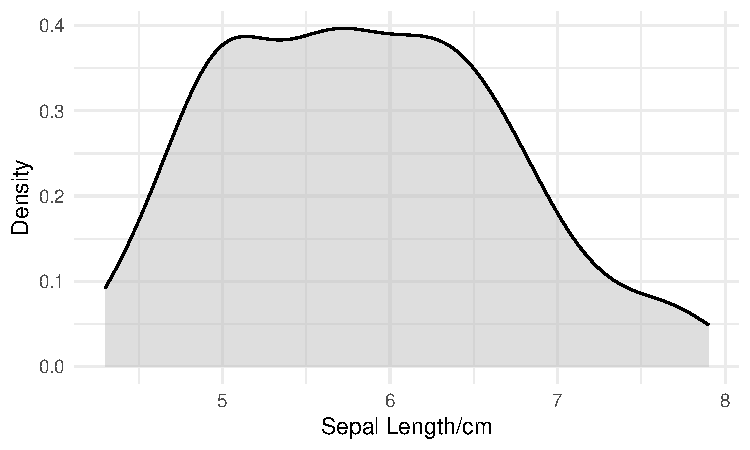
\includegraphics[width=\maxwidth]{figure/kde3-1} \caption[Kernel Density Estimation of Sepal Length in Iris Dataset]{Kernel Density Estimation of Sepal Length in Iris Dataset}\label{fig:kde3}
\end{figure}

\end{knitrout}
In figure~\ref{fig:kde3} we present the kernel density estimation of our dataset. The kernel density curve will display the distribution of sepal lengths. The peaks of the curve correspond to the main concentration trends of sepal length in the data. If the curve is unimodal, it means that the sepal lengths of most irises are concentrated in that region; if it is bimodal or multimodal, this indicates the presence of multiple such concentration areas.


\subsection{Heatmaps and Tree Maps}
In this chapter, we explore two powerful data visualisation techniques: heatmaps and treemaps. These methods are instrumental for conveying intricate data structures and patterns, offering unique ways to represent multivariate information, making them indispensable tools for data scientists.
\\  
\\We will delve into the theory behind heatmaps and treemaps, understand how to create them using popular data visualisation libraries, and demonstrate their practical applications with real-world examples. By the end of this chapter, you will be well-equipped to leverage heatmaps and treemaps to gain insights from complex and hierarchical datasets.
\subsubsection{Heatmaps - Fire in Brazil}
\\  
\\The heatmap is a data visualisation technique that uses colour coding to represent different intensity.
\\  
\\In this illustrative example, heatmaps are used to visualise fire occurrences in Brazil. These heatmaps provide a spatially coherent representation, highlighting regions at high risk and seasonal patterns. Here, the heatmap is a powerful tool for identifying the occurrence of fire incidents. The data-driven insights could empower policymakers to make informed decisions regarding preventive measures and firefighting strategies.
\\  
\\In Figure~\ref{fig:spacetime-fy22}, it can be observed that significantly higher fire counts are found in certain locations. The presence of two strips with high frequencies of fires are highly unusual.  The vertical trend corresponds to the location of BR-230 (Trans-Amazonian Highway) passing through the city of Apuí, State of Amazonas, where a high frequency of fire occurrence is observed.  The horizontal trend corresponds to BR-163 (Brazil highway) passing through Três Pinheiros in Novo Progresso, State of Pará. The western coastal area with a high frequency of fire occurrence corresponds to regions in close proximity to the cities of Vista Alegre do Abunã and Rio Branco. Research has indicated that 95 \% of active fires and the most intense ones (FRP > 500 megawatts) occurred at the edges in forests.
\\  
\\From the same figure, it can be observed that August and September are the riskiest months in terms of fire hazard, whereas little risk is posed from November to July. The follow-up question naturally arises: How does FY22 compare to previous years? Is it valid to claim that August and September constitute the fire hazard season?
\\    
\\In Figure~\ref{fig:fire-by-months-fy13-22}, the data shows a higher number of fire occurrences in the months of August to October compared to the rest of the year, indicating a greater number of fire hazards during these months.
\\  






\begin{knitrout}
\definecolor{shadecolor}{rgb}{0.969, 0.969, 0.969}\color{fgcolor}\begin{kframe}
\begin{alltt}
\hlcom{# Obtain the Brazil map data}
\hlstd{brazil_map} \hlkwb{<-} \hlkwd{map_data}\hlstd{(}\hlstr{"world"}\hlstd{,} \hlkwc{region} \hlstd{=} \hlstr{"Brazil"}\hlstd{)}

\hlcom{# Create the heatmap of fire occurrences}
\hlstd{space_heatmap} \hlkwb{<-} \hlkwd{ggplot}\hlstd{(confident_fire_fy22,} \hlkwd{aes}\hlstd{(}\hlkwc{x} \hlstd{= longitude,} \hlkwc{y} \hlstd{= latitude))} \hlopt{+}
  \hlkwd{geom_polygon}\hlstd{(}\hlkwc{data} \hlstd{= brazil_map,} \hlkwd{aes}\hlstd{(}\hlkwc{x} \hlstd{= long,} \hlkwc{y} \hlstd{= lat,} \hlkwc{group} \hlstd{= group),}
               \hlkwc{fill} \hlstd{=} \hlstr{"#bdbdbd"}\hlstd{)} \hlopt{+}
  \hlkwd{geom_bin2d}\hlstd{(}\hlkwc{bins} \hlstd{=} \hlnum{300}\hlstd{)} \hlopt{+}
  \hlkwd{scale_fill_gradient}\hlstd{(}\hlkwc{low} \hlstd{=} \hlstr{"#fee6ce"}\hlstd{,} \hlkwc{high} \hlstd{=} \hlstr{"#d7301f"}\hlstd{)} \hlopt{+}
  \hlkwd{coord_fixed}\hlstd{(}\hlkwc{ratio} \hlstd{=} \hlnum{1}\hlstd{)} \hlopt{+}
  \hlkwd{theme_minimal}\hlstd{()}\hlopt{+}
  \hlkwd{theme}\hlstd{(}\hlkwc{axis.text} \hlstd{=} \hlkwd{element_text}\hlstd{(}\hlkwc{size} \hlstd{=} \hlnum{9}\hlstd{))}

\hlstd{interactive_plot} \hlkwb{<-} \hlkwd{ggplotly}\hlstd{(space_heatmap)}

\hlstd{time_heatmap} \hlkwb{<-} \hlkwd{ggplot}\hlstd{(confident_fire_months_fy22,}
                       \hlkwd{aes}\hlstd{(}\hlkwc{x} \hlstd{= abb_month,} \hlkwc{y} \hlstd{=} \hlkwd{as.character}\hlstd{(}\hlnum{2022}\hlstd{),} \hlkwc{fill} \hlstd{= count))} \hlopt{+}
  \hlkwd{geom_tile}\hlstd{(}\hlkwc{width} \hlstd{=} \hlnum{0.9}\hlstd{,} \hlkwc{height} \hlstd{=} \hlnum{0.5}\hlstd{)} \hlopt{+}  \hlcom{# Create the heatmap tiles}
  \hlkwd{scale_fill_gradient}\hlstd{(}\hlkwc{low} \hlstd{=} \hlstr{"#fff7ec"}\hlstd{,} \hlkwc{high} \hlstd{=} \hlstr{"#d7301f"}\hlstd{)} \hlopt{+}
  \hlkwd{labs}\hlstd{(}\hlkwc{x} \hlstd{=} \hlstr{" "}\hlstd{,} \hlkwc{y} \hlstd{=} \hlstr{" "}\hlstd{,} \hlkwc{name} \hlstd{=} \hlstr{"count"}\hlstd{)} \hlopt{+}
  \hlkwd{theme_minimal}\hlstd{()} \hlopt{+}
  \hlkwd{theme}\hlstd{(}\hlkwc{axis.text} \hlstd{=} \hlkwd{element_text}\hlstd{(}\hlkwc{size} \hlstd{=} \hlnum{9}\hlstd{))}

\hlstd{spacetime_fy22} \hlkwb{<-} \hlkwd{grid.arrange}\hlstd{(space_heatmap, time_heatmap,} \hlkwc{nrow} \hlstd{=} \hlnum{2}\hlstd{,}
                               \hlkwc{heights} \hlstd{=} \hlkwd{c}\hlstd{(}\hlnum{2}\hlstd{,}\hlnum{0.5}\hlstd{))}

\hlkwd{print}\hlstd{(spacetime_fy22)}
\end{alltt}
\begin{verbatim}
## TableGrob (2 x 1) "arrange": 2 grobs
##   z     cells    name           grob
## 1 1 (1-1,1-1) arrange gtable[layout]
## 2 2 (2-2,1-1) arrange gtable[layout]
\end{verbatim}
\end{kframe}\begin{figure}
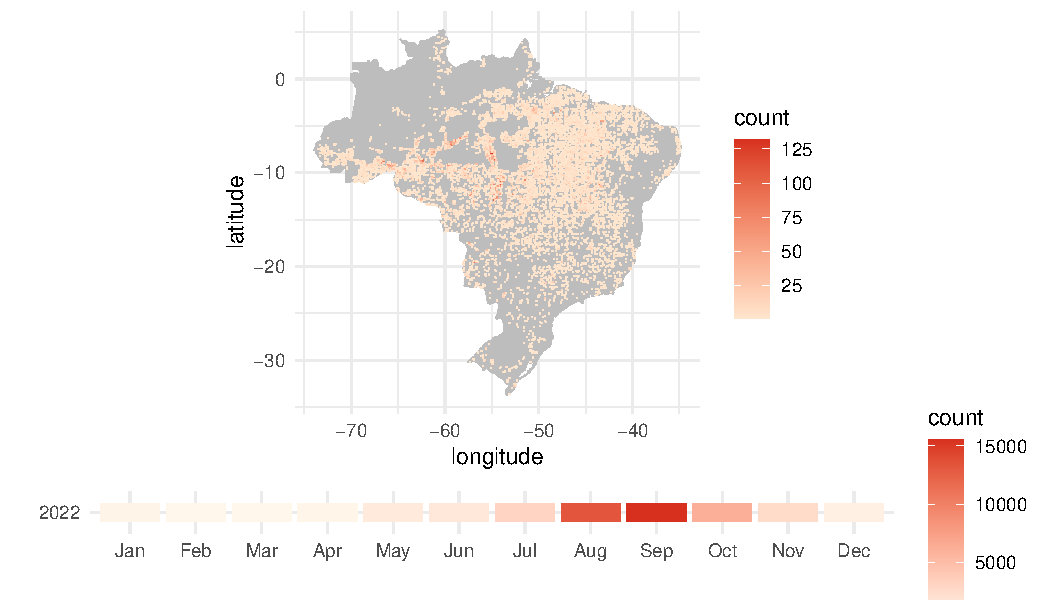
\includegraphics[width=\maxwidth]{figure/spacetime-fy22-1} \caption[Frequency of Fire by Space and Time, FY22]{Frequency of Fire by Space and Time, FY22}\label{fig:spacetime-fy22}
\end{figure}

\end{knitrout}




\begin{knitrout}
\definecolor{shadecolor}{rgb}{0.969, 0.969, 0.969}\color{fgcolor}\begin{kframe}
\begin{alltt}
\hlstd{heatmap_plot} \hlkwb{<-} \hlkwd{ggplot}\hlstd{(pivot_table,}
                       \hlkwd{aes}\hlstd{(}\hlkwc{x} \hlstd{=} \hlkwd{factor}\hlstd{(abb_month,} \hlkwc{levels} \hlstd{= custom_order),}
                           \hlkwc{y} \hlstd{=} \hlkwd{as.character}\hlstd{(year),} \hlkwc{fill} \hlstd{= count))} \hlopt{+}
  \hlkwd{geom_tile}\hlstd{()} \hlopt{+}
  \hlkwd{scale_fill_gradient}\hlstd{(}\hlkwc{low} \hlstd{=} \hlstr{"#fff7ec"}\hlstd{,} \hlkwc{high} \hlstd{=} \hlstr{"#d7301f"}\hlstd{)} \hlopt{+}
  \hlkwd{labs}\hlstd{(}\hlkwc{x} \hlstd{=} \hlstr{" "}\hlstd{,} \hlkwc{y} \hlstd{=} \hlstr{" "}\hlstd{)} \hlopt{+}
  \hlkwd{theme_minimal}\hlstd{()} \hlopt{+}
  \hlkwd{theme}\hlstd{(}\hlkwc{axis.text} \hlstd{=} \hlkwd{element_text}\hlstd{(}\hlkwc{size} \hlstd{=} \hlnum{9}\hlstd{))}

\hlkwd{print}\hlstd{(heatmap_plot)}
\end{alltt}
\end{kframe}\begin{figure}
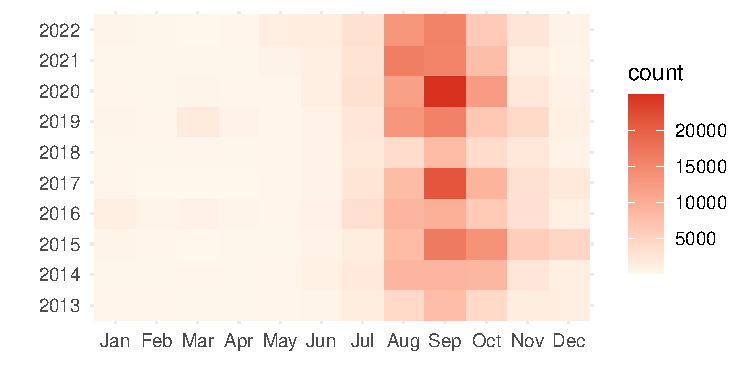
\includegraphics[width=\maxwidth]{figure/fire-by-months-fy13-22-1} \caption[Frequency of Fire Occurrences, FY13-22]{Frequency of Fire Occurrences, FY13-22}\label{fig:fire-by-months-fy13-22}
\end{figure}

\end{knitrout}


\subsubsection{Heatmaps, correlation matrix and AIC score}
\\  
\\The foundation of a heatmap is a data matrix $M$, where each entry in this matrix represents an observation:
$$M =
\left[
\begin{array}{cccc}
    M_{11} & M_{12} & \ldots & M_{1j} \\  
    M_{21} & M_{22} & \ldots & M_{2j} \\  
    \vdots & \vdots & \ddots & \vdots \\  
    M_{i1} & M_{i2} & \ldots & M_{ij}
\end{array}
\right].
$$
\\Therefore, the first step to create a heatmap is to organize the data into columns and rows. In Figure~\ref{fig:fire-by-months-fy13-22}, the structured data is displayed as a grid of coloured cells, where the colour intensity corresponds to the underlying frequency.
\\  
\\Heatmaps serve as powerful tools for visualizing relationships between covariables within a model. An example of the necessity to analyze a matrix of correlations between variables is found in regression models. In the real world, variables are often correlated, and completely independent relationships are seldom encountered. Therefore, the analysis of pairwise correlations becomes essential. Significantly impacted by highly correlated variables, the regression model requires the selection of one variable from the correlated set. The selection is based on the identification of a regression model with the lowest Akaike Information Criterion (AIC) score among these variables: 

$$AIC = -2 \l(\hat{\mathbf{\theta}})+2 \dim (\mathbf{\theta}),$$
\\where $\l(\hat{\mathbf{\theta}})$ is the log-likelihood function, which is used to find the Maximum Likelihood Estimator (MLE) of a distribution.
\\  
\\The AIC measures the extent to which the linear model fits the dataset. To obtain the best model, minimise the AIC score. In other words, the objective is to have the trend explained by the regression model, while avoiding overfitting that captures the noise in the dataset, ultimately leading to inaccurate predictions.

\subsubsection{Treemaps}
Treemaps are a visualisation method specifically designed for hierarchical data structures. They represent data as nested rectangles, where each rectangle represents a part of the whole. Treemaps offer a visually appealing and efficient way to convey the hierarchical composition of data. The size and color of each rectangle can be used to encode additional information.

\subsubsection{Use Cases for Treemaps}
Treemaps are highly effective when dealing with hierarchical data. Some common use cases include:
\begin{itemize}
\item \textbf{Disk Space Visualisation}: Treemaps can be employed to visualise disk space usage, where the outermost rectangle represents the entire disk, and inner rectangles represent folders and files. The size of each rectangle reflects the space they occupy.
\item \textbf{Market Share Analysis}: In business, treemaps are useful for visualizing market share data. The top-level rectangle represents the total market, and inner rectangles represent individual segments, brands, or products. The size and color of each segment can represent its share and performance.
\end{itemize}

XXX %missing Treemaps


\subsection{Line Charts and Time Series Visualisation}

In this chapter, we are going to investigate the intricacies of the line chart and its most common application: time series.\\
First, a line chart is a statistical representation that uses a Cartesian coordinate system, where each point on the chart corresponds to a pair of coordinates $(x,y)$, to depict changes in numerical values over continuous time intervals or ordered categories. The x-axis typically represents these intervals or categories, while the y-axis conveys quantified data. Hence, data points, represented by a coordinates $\{(x_i,y_i)\}_{1 \leq i \leq n}$, $n$ being the total number of data points. In a line chart, consecutive data points are typically connected by straight lines. The line segment between two points $(x_i,y_i)$ and $(x_{i+1},y_{i+1})$ can be described by the equation of a line in the slope-intercept form: $y=mx+b$, where $m$ is the slope and $b$ is the y-intercept.

\subsubsection{Suitability for Displaying Trends Over Time}
Line charts effectively visualise data trends over time. By plotting data at intervals like days or years, they highlight trends and patterns. Multiple lines on one chart enable easy data comparison, such as contrasting sales of two products. They aid in recognizing seasonal changes, cyclic events, and unexpected shifts, making them invaluable for forecasting. Due to their simplicity, they're accessible to those with minimal data analysis background. Line charts are a prime choice for time series visualisation.

Time series visualisation is essential in data analysis, showcasing time-ordered data. It reveals long-term trends, helping analysts discern patterns for future planning. It's crucial for spotting seasonality in datasets. This method also identifies anomalies, suggesting areas needing investigation. Predictive modeling, based on historical patterns, becomes feasible, fostering proactive choices. Overlaying multiple data series offers richer comparative analysis. Overall, time series visualisation provides quick insights into chronological data, driving informed decisions by highlighting trends, seasonal changes, and outliers.\\
\noindent
\textbf{Limitations:}\\
While line charts are excellent for displaying trends over time, they have limitations. They may not be suitable for showing individual data distributions or for data where there's no logical order. eg. too many points, too many lines, too many zeros.

\subsubsection{Showcase real-world examples of time series visualisations}

Here, we are going to investigate 'exchange rate dataset' and plot all daily and 21-day moving average exchange rates in one figure.





\begin{figure}
\begin{knitrout}
\definecolor{shadecolor}{rgb}{0.969, 0.969, 0.969}\color{fgcolor}\begin{kframe}
\begin{alltt}
\hlcom{# Plot daily and 21-day moving average exchange rates of CNY, CAN,}
\hlcom{# EUR, HKD, USD to GBP}

\hlcom{# First plot}
\hlstd{p1} \hlkwb{<-} \hlkwd{ggplot}\hlstd{(plot_dt,} \hlkwd{aes}\hlstd{(}\hlkwc{x}\hlstd{=Date,} \hlkwc{y}\hlstd{=Rate,} \hlkwc{color}\hlstd{=Currency))} \hlopt{+} \hlkwd{geom_line}\hlstd{()} \hlopt{+}
  \hlkwd{labs}\hlstd{(}\hlkwc{title}\hlstd{=}\hlstr{"Daily exchange rates"}\hlstd{,} \hlkwc{y}\hlstd{=}\hlstr{"Exchange Rate to GBP"}\hlstd{,}
       \hlkwc{x}\hlstd{=}\hlstr{"Date"}\hlstd{,} \hlkwc{color}\hlstd{=}\hlstr{"Currency"}\hlstd{)}\hlopt{+}
  \hlkwd{theme_minimal}\hlstd{()} \hlopt{+} \hlkwd{theme}\hlstd{(}\hlkwc{legend.position}\hlstd{=}\hlstr{"none"}\hlstd{)}

\hlcom{# Second plot}
\hlstd{p2} \hlkwb{<-} \hlkwd{ggplot}\hlstd{(plot_data,} \hlkwd{aes}\hlstd{(}\hlkwc{x}\hlstd{=Date,} \hlkwc{y}\hlstd{=Rate,} \hlkwc{color}\hlstd{=Currency))} \hlopt{+} \hlkwd{geom_line}\hlstd{()} \hlopt{+}
  \hlkwd{labs}\hlstd{(}\hlkwc{title}\hlstd{=}\hlstr{"21-Day moving average \textbackslash{}n exchange rates"}\hlstd{,}
       \hlkwc{y}\hlstd{=}\hlstr{"Exchange Rate to GBP"}\hlstd{,} \hlkwc{x}\hlstd{=}\hlstr{"Date"}\hlstd{,} \hlkwc{color}\hlstd{=}\hlstr{"Currency"}\hlstd{)}\hlopt{+}
  \hlkwd{theme_minimal}\hlstd{()} \hlopt{+} \hlkwd{theme}\hlstd{(}\hlkwc{legend.position}\hlstd{=}\hlstr{"none"}\hlstd{)}

\hlcom{# Extract the legend}
\hlstd{p2_legend} \hlkwb{<-} \hlstd{cowplot}\hlopt{::}\hlkwd{get_legend}\hlstd{(p2} \hlopt{+} \hlkwd{theme}\hlstd{(}\hlkwc{legend.position}\hlstd{=}\hlstr{"bottom"}\hlstd{))}
\hlcom{# Combine the plots with adjusted widths using cowplot}
\hlstd{combined_plot} \hlkwb{<-} \hlstd{cowplot}\hlopt{::}\hlkwd{plot_grid}\hlstd{(p1, p2,} \hlkwc{labels} \hlstd{=} \hlkwd{c}\hlstd{(}\hlstr{"1"}\hlstd{,} \hlstr{"2"}\hlstd{),}
                                    \hlkwc{rel_widths} \hlstd{=} \hlkwd{c}\hlstd{(}\hlnum{1}\hlstd{,} \hlnum{1}\hlstd{),} \hlkwc{nrow}\hlstd{=}\hlnum{1}\hlstd{)}
\hlcom{# Combine the plots and the legend}
\hlstd{cowplot}\hlopt{::}\hlkwd{plot_grid}\hlstd{(combined_plot, p2_legend,} \hlkwc{ncol}\hlstd{=}\hlnum{1}\hlstd{,} \hlkwc{rel_heights} \hlstd{=} \hlkwd{c}\hlstd{(}\hlnum{1}\hlstd{,} \hlnum{.1}\hlstd{))}
\end{alltt}
\end{kframe}
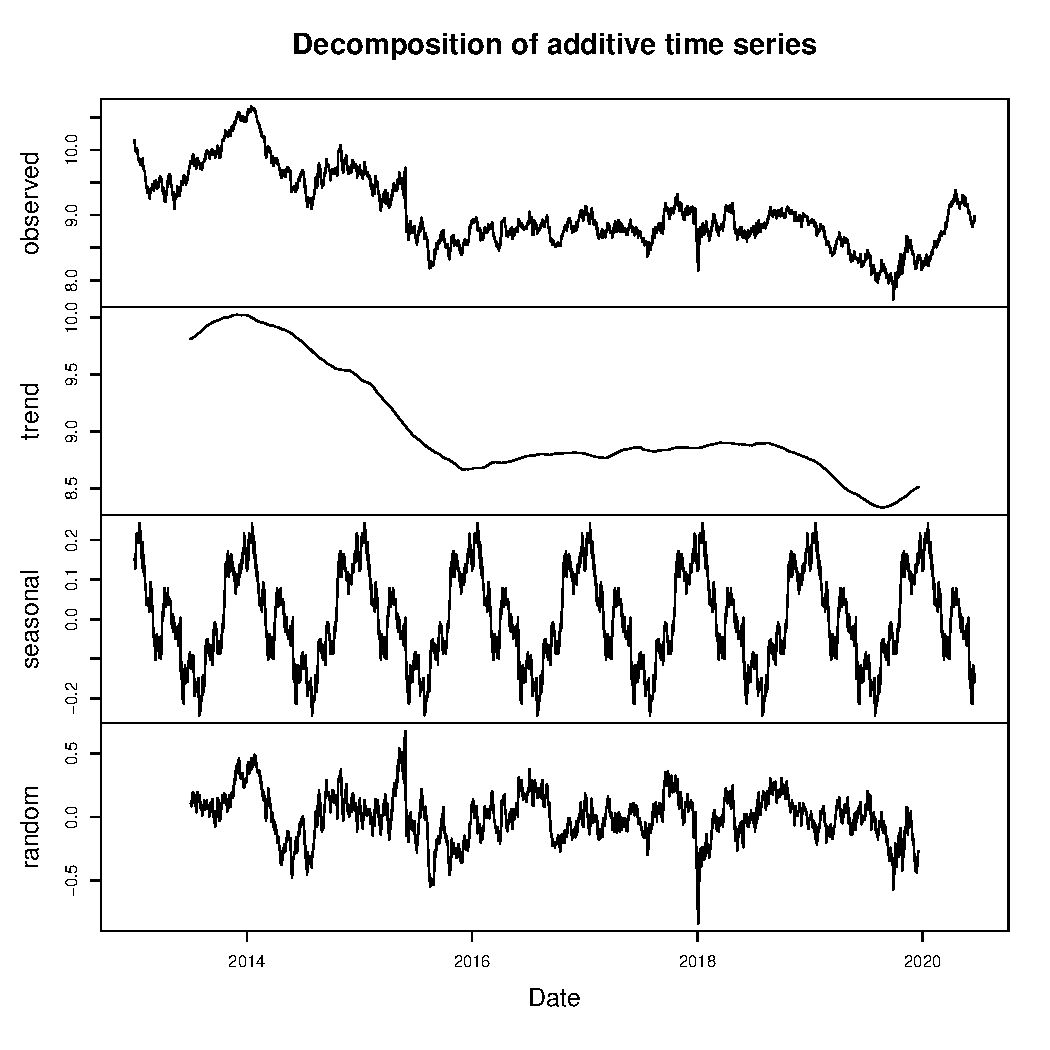
\includegraphics[width=\maxwidth]{figure/unnamed-chunk-2-1} 
\end{knitrout}
\centering
\caption{Daily and 21-day moving average exchange rates of CNY, CAN, EUR, HKD, USD to GBP}
\label{fig:all exchange rates}
\end{figure}


From the first plot of Figure~\ref{fig:all exchange rates}, we can see the the daily CNY, CAN, EUR, HKD, USD versus GBP exchange in the same plot, which provide us an overview of the trend and comparison. Then we can make the plot smooth by taking averages, which enables easier recognition of trend. From second plot, utilizing a 21-day moving average to represent several exchange rates offers multiple benefits. Firstly, it smoothens out short-term fluctuations, providing a clearer view of the underlying trend in the exchange rates. This helps in identifying consistent patterns and removes noise caused by daily volatility. Secondly, when applied to multiple exchange rates, it allows for a standardized comparison between them.

However, from Figure~\ref{fig:all exchange rates}, for example there are huge gaps between "CNYtoGBP" and "EURtoGBP". This may not suitable for viewing their trends simutaneosly. If we want to display two different time series that measure two different quantities at the same time points, we can draw the second series again on the second Y-axis on the right side.


\begin{figure}[H]
\begin{knitrout}
\definecolor{shadecolor}{rgb}{0.969, 0.969, 0.969}\color{fgcolor}\begin{kframe}
\begin{alltt}
\hlcom{# Plot Double y-axis time series of CNY and EUR to GBP}
\hlcom{# Define scale factor}
\hlstd{scale_factor} \hlkwb{<-} \hlkwd{max}\hlstd{(MyData}\hlopt{$}\hlstd{CNYtoGBP)} \hlopt{/} \hlkwd{max}\hlstd{(MyData}\hlopt{$}\hlstd{EURtoGBP)}
\hlstd{df} \hlkwb{<-} \hlstd{MyData} \hlopt \hlkwd{select}\hlstd{(Date,CNYtoGBP, EURtoGBP)}

\hlcom{# Create plot with dual y-axes}
\hlkwd{ggplot}\hlstd{(df,} \hlkwd{aes}\hlstd{(Date))} \hlopt{+} \hlkwd{geom_line}\hlstd{(}\hlkwd{aes}\hlstd{(}\hlkwc{y} \hlstd{= EURtoGBP,} \hlkwc{color} \hlstd{=} \hlstr{"EURtoGBP"}\hlstd{))}\hlopt{+}
  \hlkwd{geom_line}\hlstd{(}\hlkwd{aes}\hlstd{(}\hlkwc{y} \hlstd{= CNYtoGBP} \hlopt{/} \hlstd{scale_factor,} \hlkwc{color} \hlstd{=} \hlstr{"CNYtoGBP"}\hlstd{))}\hlopt{+}
  \hlkwd{scale_y_continuous}\hlstd{(}\hlkwc{name} \hlstd{=} \hlstr{"EURtoGBP Exchange Rate axis"}\hlstd{,}
                     \hlkwc{sec.axis} \hlstd{=} \hlkwd{sec_axis}\hlstd{(}\hlopt{~} \hlstd{.} \hlopt{*} \hlstd{scale_factor,}
                                         \hlkwc{name} \hlstd{=} \hlstr{"CNYtoGBP Exchange Rate axis"}\hlstd{))}\hlopt{+}
  \hlkwd{labs}\hlstd{(}\hlkwc{color} \hlstd{=} \hlstr{"Currency"}\hlstd{)} \hlopt{+} \hlkwd{theme_minimal}\hlstd{()} \hlopt{+} \hlkwd{theme}\hlstd{(}\hlkwc{legend.position}\hlstd{=}\hlstr{"bottom"}\hlstd{)}
\end{alltt}
\end{kframe}
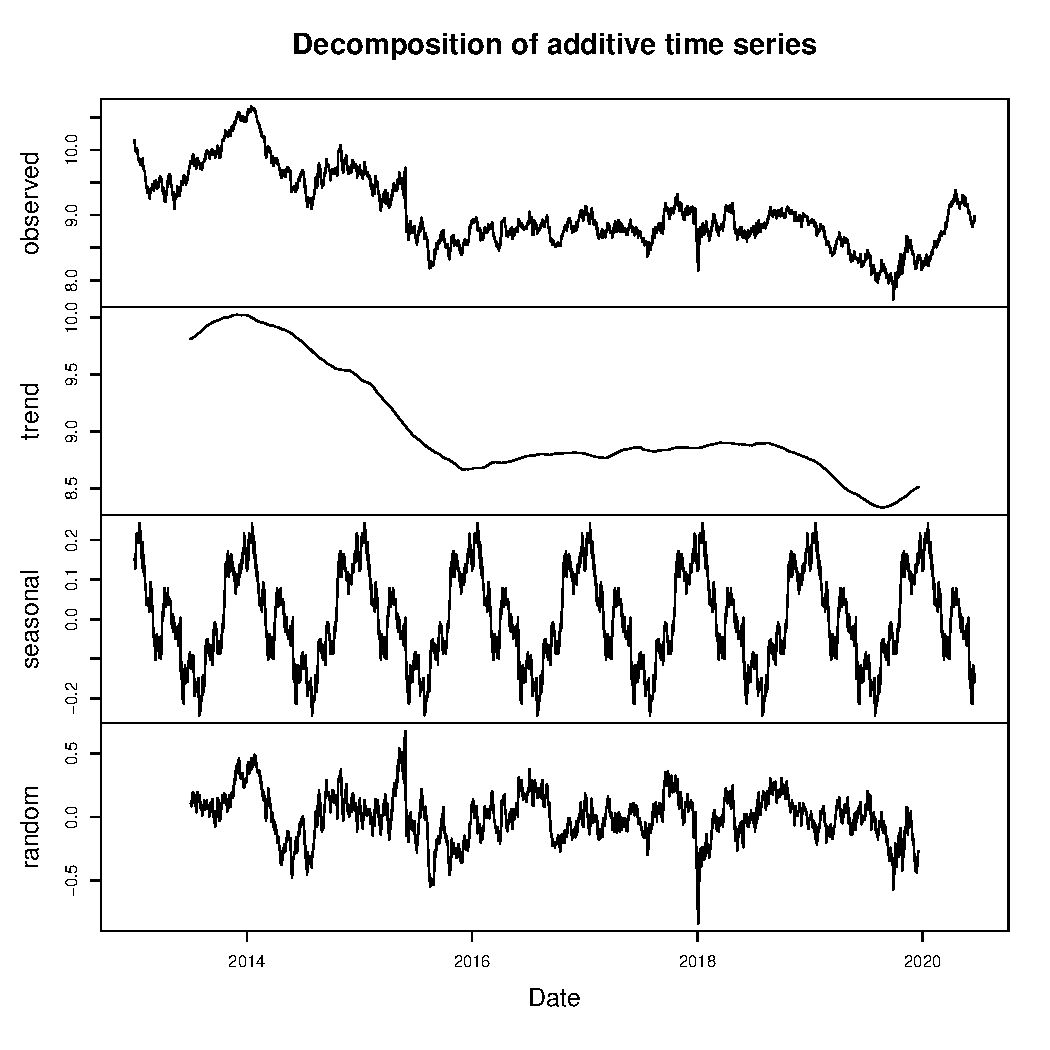
\includegraphics[width=\maxwidth]{figure/unnamed-chunk-3-1} 
\end{knitrout}
\centering
\caption{Double y-axis time series of CNY and EUR to GBP}
\label{fig:Double y-axis}
\end{figure}


From Figure~\ref{fig:Double y-axis}, the left y-axis represents spot exchange rate of EUR against GBP and the right one represents spot exchange rate of CNY against GBP. Using a double Y-axis to represent the spot exchange rates of EUR to GBP and CNY to GBP offers several advantages. It facilitates the direct comparison of trends between the two exchange rates, providing insights into their correlations or discrepancies. This method is also space-efficient, combining two data series into one graph, allowing for a more concise data presentation. By juxtaposing the two rates, analysts can discern potential global factors affecting both or highlight specific currency volatilities. Additionally, presenting both datasets together offers contextual understanding and simplifies interpretation for a general audience. However, care must be taken with scale selection to avoid potential misrepresentation or misinterpretation.
\\
\noindent
\textbf{Decomposition of one time series into trend, seasonal, and random:}

One of the primary advantages of time series visualisation is the ease with which it allows analysts to identify long-term upward or downward trends in data and patterns that repeat over specific intervals. By decomposing the time series, it would be easy to see those features.

Time series data, $Y_t$, can often be described as a combination of several distinct components:
\begin{itemize}
    \item \textbf{Trend ($T_t$):} The underlying progression in the series.
    \item \textbf{Seasonal ($S_t$):} Periodic fluctuations due to seasonal factor.
    \item \textbf{Residual ($R_t$):} The irregular or error component.
\end{itemize}

The decomposition of a time series can be described in two main models:\\
Additive Model:
In the additive model, the components are added together:
\[
Y_t = T_t + S_t + R_t
\]
Multiplicative Model:
In the multiplicative model, the components are multiplied together:
\[
Y_t = T_t \times S_t \times R_t
\]
In practice, the choice between the additive and multiplicative models often depends on the nature of the time series. If the magnitude of the seasonal fluctuations or the variation around the trend does not vary with the level of the time series, then an additive model is appropriate. If the magnitude of the seasonal fluctuations or the variation around the trend increases or decreases as the time series level changes, then a multiplicative model may be more suitable.


\begin{figure}[H]
\begin{knitrout}
\definecolor{shadecolor}{rgb}{0.969, 0.969, 0.969}\color{fgcolor}\begin{kframe}
\begin{alltt}
\hlcom{# Plot decomposition of addictive time series model}
\hlstd{decomposed_ts} \hlkwb{<-} \hlstd{stats}\hlopt{::}\hlkwd{decompose}\hlstd{(ts_data}\hlopt{$}\hlstd{CNYtoGBP)}
\hlkwd{plot}\hlstd{(decomposed_ts,} \hlkwc{xlab}\hlstd{=}\hlstr{"Date"}\hlstd{)}
\end{alltt}
\end{kframe}
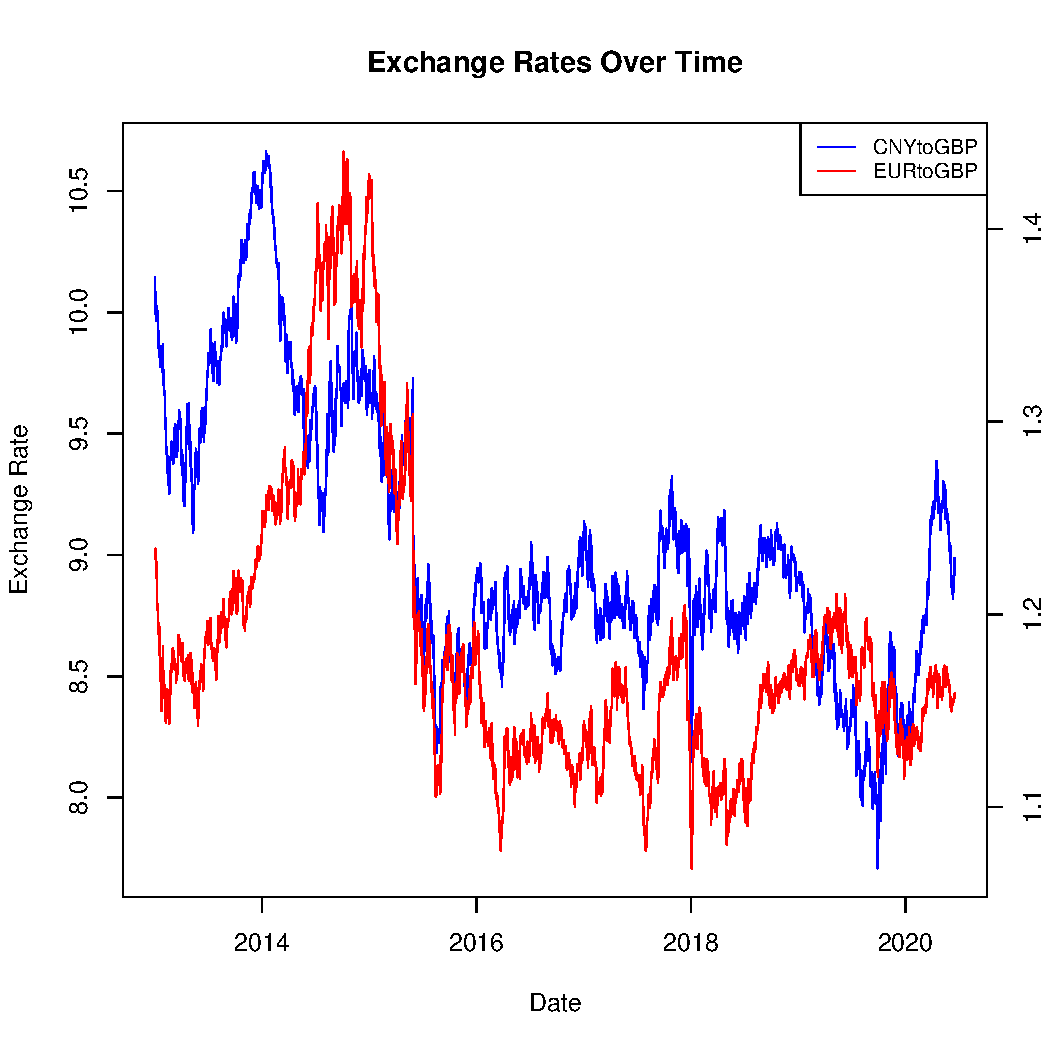
\includegraphics[width=\maxwidth]{figure/unnamed-chunk-4-1} 
\end{knitrout}
\centering
\caption{Decomposition of addictive time series model of CNY to GBP exchange rates}
\label{fig:decomposition of time series}
\end{figure}


Hence, in this way, we will be able to view the seasonal trend and overall trend of CNY to GBP obviously. From Figure~\ref{fig:decomposition of time series}, we can see that the spot exchange rate of CNY to GBP is gradually decreasing as time goes and it has a cyclical trend during years.


\subsection{Network Graphs}
\textbf{Definition and Utility:}
Network graphs, often referred to as graphs or networks, are a powerful data visualisation method used to depict relationships between entities. These entities, known as nodes, are interconnected by edges or links, which represent relationships, connections, or interactions. Network graphs find extensive utility in various fields, such as social network analysis, transportation systems, and even biological networks like protein-protein interactions. They excel at revealing complex dependencies and structures, making them a critical tool for understanding relational data.

\subsubsection{The Mathematics behind Network Graphs:}
Constructing network graphs involves several mathematical intricacies. Here we present just a few of the many concepts that play a role in the creation of such graphs:
\begin{enumerate}
\item \textbf{Nodes and Edges}: Mathematically, a network graph, \(G\), is defined as \(G = (V, E)\), where \(V\) represents the set of nodes and \(E\) represents the set of edges connecting these nodes.
\item \textbf{Node Degree}: The degree of a node is the number of edges connected to it. In a directed graph, nodes can have both in-degrees and out-degrees.
\item \textbf{Centrality Measures}: Centrality metrics like degree centrality, betweenness centrality, and closeness centrality provide insights into the relative importance or influence of nodes within a network.
\item \textbf{Graph Metrics}: Graph theory concepts like shortest paths, connected components, and clustering coefficients are used to analyze the network's structure.
\end{enumerate}

\textbf{Formulas used in Network Graphs:}

\begin{enumerate}
\item \textbf{Degree of a Node (Undirected Graph)}:
\[
\text{Degree}(v) = \sum_{w \in V} A(v, w)
\]
where \(A(v, w)\) is the adjacency matrix element, indicating whether there is a connection between nodes \(v\) and \(w\).
\item \textbf{Degree of a Node (Directed Graph)}:
\[
\text{In-Degree}(v) = \sum_{w \in V} A(w, v)
\]
\[
\text{Out-Degree}(v) = \sum_{w \in V} A(v, w)
\]
\item \textbf{Betweenness Centrality (for unweighted graphs)}:
\[
C_B(v) = \sum_{s \neq v \neq t} \frac{\sigma_{st}(v)}{\sigma_{st}}
\]
where \(\sigma_{st}\) is the number of shortest paths from node \(s\) to \(t\), and \(\sigma_{st}(v)\) is the number of those paths passing through node \(v\).
\end{enumerate}

\subsubsection{Network Graphs in Practice}




\begin{figure}[h]
\centering
\begin{knitrout}
\definecolor{shadecolor}{rgb}{0.969, 0.969, 0.969}\color{fgcolor}\begin{kframe}
\begin{alltt}
\hlcom{# Plot the graph}
\hlcom{#plot(lesmis_graph, layout = layout, vertex.label.cex = 0.7, main = "Character Interactions in Les Misérables")}
\end{alltt}
\end{kframe}
\end{knitrout}
\end{figure}

\subsection{Sankey Diagrams}
xxx

\subsection{Geographic Maps and Spatial Data Visualisation}

A \textbf{geographical maps} is a visual representation of an area—a symbolic depiction highlighting relationships between elements of that space, such as objects, regions, or themes. Maps have been used for centuries to navigate and explore the world, and they play a crucial role in understanding our environment, both locally and globally. These maps serve as canvases on which spatial data is painted, allowing for a visual comprehension of information that might otherwise remain abstract.

Before moving on to the spatial data visualisation. It is essential to understand how we map the the earth on a plane. The Earth, a three-dimensional spheroid, can be transformed on a plane through map projections. Each projection offers a different way to "flatten" the Earth, and as a result, each has its strengths and distortions. For instance, the Mercator projection preserves angles but distorts areas as you move towards the poles. Beyond projections, coordinate systems, like the commonly used latitude and longitude, provide a standardized way to pinpoint any location on Earth.

\begin{itemize}
\item \textbf{Latitude} measures the angle between a point on the Earth's surface and the equator, moving north or south. And latitude values range from -90° (South Pole) to +90° (North Pole). The equator, which divides the Earth into the Northern and Southern Hemispheres, is at 0° latitude.
\item \textbf{Longitude} measures the angle between a point on the Earth's surface and the prime meridian, moving east or west.
And longitude values range from -180° to +180°. The prime meridian, which is at 0° longitude, runs from the North Pole through Greenwich, England, to the South Pole. It divides the Earth into the Eastern and Western Hemispheres.
\end{itemize}

Together, lines of longitude and latitude create a grid system over the Earth's surface. By providing both a latitude and longitude value, one can specify an exact location on the Earth's surface. For example, the coordinates (0° N, 0° E) would indicate the intersection of the equator and the prime meridian, located in the Gulf of Guinea off the west coast of Africa.
\\\\
\noindent
\textbf{Spatial data visualisation}\\
Spatial data visualisation are powerful tools that transform raw, often complex datasets into visual representations, revealing patterns, relationships, and insights rooted in location. At their core, maps provide a spatial context, allowing us to see the world's intricate web of interconnectedness. Today, with the surge in big data and advanced visualisation tools, spatial data visualisation is not just about presenting information but also about telling compelling stories, guiding decision-making, and predicting future trends based on geographical patterns.



\noindent
Here, we are going to construct a geographical map of the Greater London and show each ward. 



\begingroup
\setlength{\intextsep}{5pt plus 2pt minus 2pt}
\setlength{\textfloatsep}{5pt plus 2pt minus 2pt}
\setlength{\abovecaptionskip}{2pt plus 1pt minus 1pt}
\setlength{\belowcaptionskip}{2pt plus 1pt minus 1pt}

\begin{figure}[H]
\begin{knitrout}
\definecolor{shadecolor}{rgb}{0.969, 0.969, 0.969}\color{fgcolor}\begin{kframe}
\begin{alltt}
\hlcom{# Plot London map by ward}
\hlkwd{ggplot}\hlstd{(}\hlkwc{data} \hlstd{= london_boroughs)} \hlopt{+} \hlkwd{geom_sf}\hlstd{(}\hlkwc{fill} \hlstd{=} \hlstr{"lightblue"}\hlstd{,} \hlkwc{color} \hlstd{=} \hlstr{"black"}\hlstd{)} \hlopt{+}
  \hlkwd{theme_minimal}\hlstd{()} \hlopt{+} \hlkwd{labs}\hlstd{(}\hlkwc{y}\hlstd{=}\hlstr{"Latitude"}\hlstd{,} \hlkwc{x}\hlstd{=}\hlstr{"Longitude"}\hlstd{)}
\end{alltt}
\end{kframe}
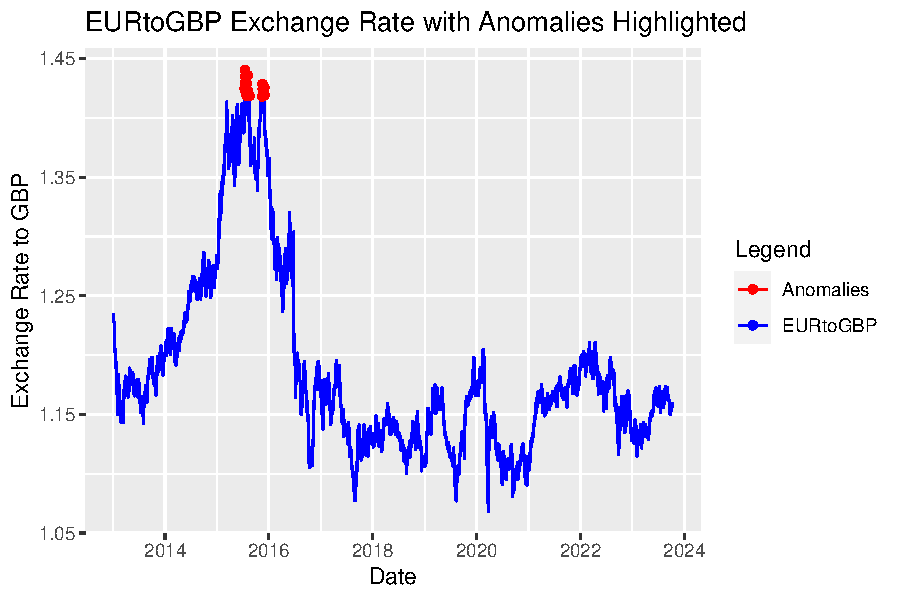
\includegraphics[width=\maxwidth]{figure/unnamed-chunk-6-1} 
\end{knitrout}
\centering
\caption{London Wards Map}
\label{fig:London Wards Map}
\end{figure}
\endgroup

From Figure~\ref{fig:London Wards Map}, we can all wards of the Greater London and we can specify their locations by latitude and longitude. However, a map does not convey much information except the position. Hence, we are going to calculate the crime rate by dividing crime count in the borough by population in the borough at 2020 and present by a choropleth map.


\begin{figure}[H]
\begin{knitrout}
\definecolor{shadecolor}{rgb}{0.969, 0.969, 0.969}\color{fgcolor}\begin{kframe}
\begin{alltt}
\hlcom{# Plot the Crime rate in London by boroughs}
\hlkwd{ggplot}\hlstd{(}\hlkwc{data}\hlstd{=aggregated_data)} \hlopt{+} \hlkwd{geom_sf}\hlstd{(}\hlkwd{aes}\hlstd{(}\hlkwc{fill}\hlstd{=Crime_rate))} \hlopt{+}
  \hlkwd{geom_sf_text}\hlstd{(}\hlkwd{aes}\hlstd{(}\hlkwc{label} \hlstd{= DISTRICT,} \hlkwc{geometry} \hlstd{= centroid),}
               \hlkwc{size} \hlstd{=} \hlnum{2.5}\hlstd{,} \hlkwc{check_overlap} \hlstd{=} \hlnum{TRUE}\hlstd{)} \hlopt{+}
  \hlkwd{scale_fill_gradient}\hlstd{(}\hlkwc{low}\hlstd{=}\hlstr{"Green"}\hlstd{,} \hlkwc{high}\hlstd{=}\hlstr{"red"}\hlstd{)} \hlopt{+} \hlkwd{theme_minimal}\hlstd{()} \hlopt{+}
  \hlkwd{labs}\hlstd{(}\hlkwc{fill}\hlstd{=}\hlstr{"Crime rate"}\hlstd{)}
\end{alltt}
\end{kframe}
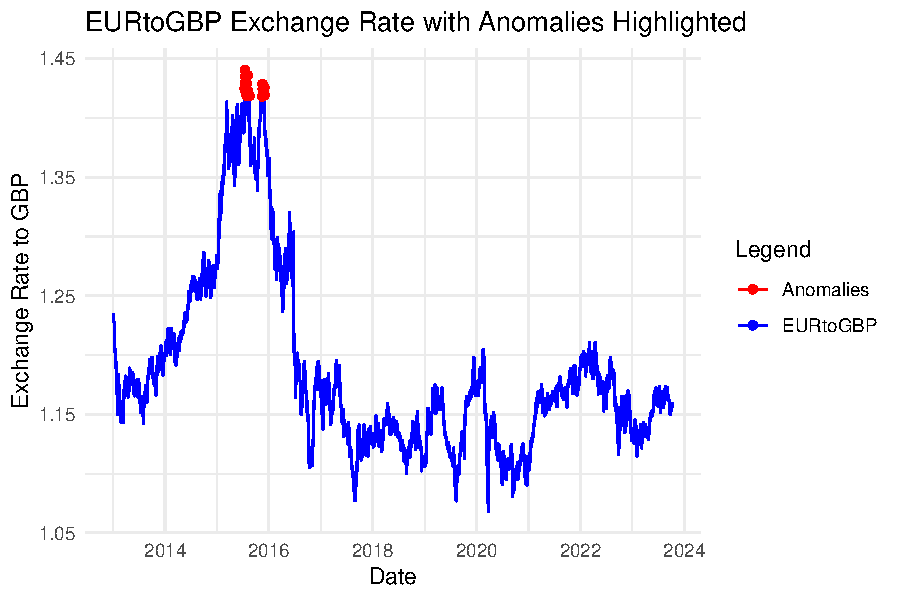
\includegraphics[width=\maxwidth]{figure/unnamed-chunk-7-1} 
\end{knitrout}
\centering
\caption{Crime rate by boroughs in London in 2020}
\label{fig:crime rate london}
\end{figure}

From Figure~\ref{fig:crime rate london}, we can discern the safety levels of each borough. Green denotes safe areas, while red indicates unsafe ones. It is evident that boroughs closer to the city center tend to be less safe.

\subsection{3D and Interactive Visualisations}
ggplot2 is one of the most popular data visualisation libraries in R, but it is primarily designed for 2D data visualisation. Directly creating 3D views with ggplot2 can be challenging.

rgl: This is a widely-used package for 3D visualisations. It allows you to create interactive 3D scatter plots, line plots, and more, and view them in a separate window.

3D data visualisation is an approach that employs three-dimensional graphics to represent complex data structures, allowing for an immersive exploration of information. Unlike traditional 2D visualisations (like bar graphs or line charts), 3D visualisations can convey an additional dimension of data, making them particularly valuable in specific contexts.

Our first example will be  a scatter plot. We can use scatterplot3d package to help us for data visualisation.
\section{Trees Dataset in R}


\begin{knitrout}
\definecolor{shadecolor}{rgb}{0.969, 0.969, 0.969}\color{fgcolor}\begin{kframe}
\begin{alltt}
\hlcom{# Generate colors based on the Volume variable}
\hlstd{colors} \hlkwb{<-} \hlkwd{colorRampPalette}\hlstd{(}\hlkwd{c}\hlstd{(}\hlstr{"blue"}\hlstd{,} \hlstr{"red"}\hlstd{))(}\hlkwd{length}\hlstd{(}\hlkwd{unique}\hlstd{(trees}\hlopt{$}\hlstd{Volume)))}
\hlstd{color_assign} \hlkwb{<-} \hlstd{colors[}\hlkwd{as.numeric}\hlstd{(}\hlkwd{as.factor}\hlstd{(trees}\hlopt{$}\hlstd{Volume))]}
\hlcom{# Create 3d scatter plot with colors}
\hlkwd{scatterplot3d}\hlstd{(trees}\hlopt{$}\hlstd{Girth, trees}\hlopt{$}\hlstd{Height, trees}\hlopt{$}\hlstd{Volume,}
              \hlkwc{color}\hlstd{=color_assign,}
              \hlkwc{main}\hlstd{=}\hlstr{"3D Scatterplot of trees data"}\hlstd{,}
              \hlkwc{xlab}\hlstd{=}\hlstr{"Girth (inches)"}\hlstd{,}
              \hlkwc{ylab}\hlstd{=}\hlstr{"Height (ft)"}\hlstd{,}
              \hlkwc{zlab}\hlstd{=}\hlstr{"Volume (cubic ft)"}\hlstd{)}
\end{alltt}
\end{kframe}\begin{figure}
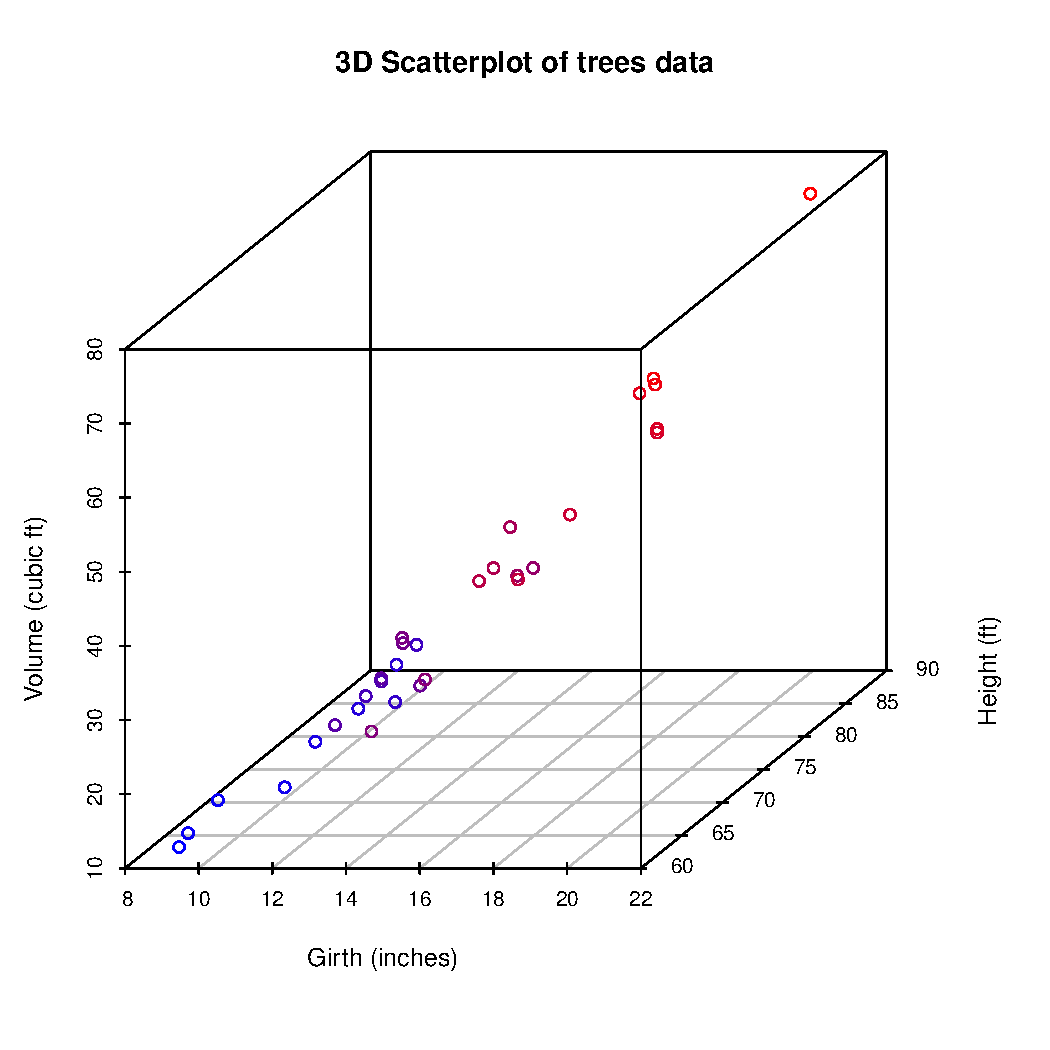
\includegraphics[width=\maxwidth]{figure/3d1-1} \caption[3d scatter plot]{3d scatter plot}\label{fig:3d1}
\end{figure}

\end{knitrout}




\subsection{Advanced Visualisation Techniques}
xxx




\section{Practical Implementations}
XXX




\section{Case Studies}
\subsection{Market Analysis Dashboards}
XXX
\subsection{Healthcare Data Visualisation}
XXX




\section{State-of-the-Art Approaches}
XXX


\section{Conclusion}

XXX

\end{document}
